%----------------------------------------------------------------------------------------
%	PACKAGES AND OTHER DOCUMENT CONFIGURATIONS
%----------------------------------------------------------------------------------------


\documentclass[12pt,openright,oneside,final]{report}
\usepackage{generators/imports}
\usepackage{tabulary}
\usepackage{float}
\usepackage{makecell}
\usepackage{pdfpages}

\restylefloat{table}
\include{generators/glossary}
\begin{document}
\begin{titlepage}

\newcommand{\HRule}{\rule{\linewidth}{0.5mm}} % Defines a new command for the horizontal lines, change thickness here

\center % Center everything on the page
 
%----------------------------------------------------------------------------------------
%	HEADING SECTIONS
%----------------------------------------------------------------------------------------

\textsc{\LARGE University of Bergen \\ Department of information science}\\[1.5cm] % Name of your university/college

%----------------------------------------------------------------------------------------
%	TITLE SECTION
%----------------------------------------------------------------------------------------

\HRule \\[0.5cm]
\begin{Huge}
	\bfseries{A social cooperative fitness application promoting an active lifestyle}\\[0.7cm] % Title of your document
\end{Huge}
\HRule \\[0.5cm]

%----------------------------------------------------------------------------------------
%	AUTHOR SECTION
%----------------------------------------------------------------------------------------

\large \emph{Author:} Kristoffer Marthinsen\\
\large \emph{Supervisor:} Duc Tien Dang Nguyen\\[2cm]

%----------------------------------------------------------------------------------------
%   LOGO SECTION
% 	This will require the graphicx package
%	Change the line to comment if you only want the UiB Logo
%	Logo for other faculties here: http://kapd.h.uib.no/profilmanual/99LastNed/99a_lastned.html
%----------------------------------------------------------------------------------------


\centerline{
\includegraphics[scale=0.15]{figures/canvas}}  %change for your faculty

%----------------------------------------------------------------------------------------
%	DATE SECTION
%----------------------------------------------------------------------------------------

{\large \monthyeardate\today}\\[3cm] % Date, change the \today to a set date if you want to be precise

%----------------------------------------------------------------------------------------
%	LOGO SECTION
%----------------------------------------------------------------------------------------

\vfill % Fill the rest of the page with whitespace

\end{titlepage}
 % This is the titlepage
\pagenumbering{roman}

\begin{abstract}
\noindent
The world health organization (WHO) lists insufficient activity as one of the leading risk factors for death worldwide. Insufficient activity can lead to many fatal cardiovascular diseases, obesity, cancer and diabetes.
The world health organization recommends that adults should do at least 150 minutes of moderate-intensity physical activity a week.  Physical activities like running, cycling, playing sports, organized exercise can decrease the health and disease risks associated with a sedentary lifestyle. 


 In this research proposal, a literature review has been done for a social cooperative fitness application that logs training data for friends, families or work place colleagues that have similar fitness goals in mind. The goal of the application is to encourage exercise and keep each member accountable of each other to promote physical health.

 The literature research suggests that having small groups consisting of friends with similar fitness goals are more motivated to exercise and the users keep each other accountable. Using leaderboards in smaller groups is also more beneficial for motivation and can lead to knowledge and information sharing between the users.
 
This research will help the field of human computer interaction to understand how users interact in a social setting while staying motivated by using technology to log their physical activities and exercise.
\end{abstract}

\renewcommand{\abstractname}{Acknowledgements}
\begin{abstract}
Shoutout to all my g`s
	
	\vspace{1cm}
	\hspace*{\fill}\texttt{Kristoffer Marthinsen}\\ 
	\hspace*{\fill} 01 June, 2020
\end{abstract}

{\tableofcontents \let\cleardoublepage\clearpage \listoffigures \let\cleardoublepage\clearpage \listoftables \let\cleardoublepage\clearpage} 
\pagenumbering{arabic}
\setcounter{page}{1}
\setlength{\parskip}{0.5cm plus4mm minus3mm}
\setlength\parindent{0pt}

\chapter{Introduction and Research Questions}
\section{Introduction}
Inactive and sedentary lifestyles are becoming a big issue around the world. “People are spending more and more time doing sedentary activities. During our leisure time, we are often sitting: while using a computer or other device, watching TV, or playing video games.”\cite{NIH}. Most of the jobs are becoming increasingly sedentary as well, as most jobs consists of long days in front of a desk. The situation is similar for the younger generation as they spend long days sitting at schools or universities. 

Sitting promotes deconditioning, which negatively affects employees’ abilities to meet the demands of increasingly physical workloads.\cite{Lurati} The average person spends a big portion of their day sitting still and prolonged sitting and sedentary lifestyles may lead to premature aging and contribute to chronic disease, prelude to lost productivity.(ibid). Not only are people sedentary, they are also inactive during their off time. An inactive lifestyle is a lifestyle with a lot of sitting and lying down with very little to no exercise \cite{NIH2} .

The world health organization (WHO) lists insufficient activity as one of the leading risk factors for death worldwide.  Insufficient activity is a key risk factor for many diseases like cardiovascular diseases, cancer and diabetes. \cite{WHO}. They state that more than 80\% of the world’s adolescent population is not active enough, and more than 25\% of the adult population. The world health organization recommends that adults should do at least 150 minutes of moderate-intensity physical activity a week.  Physical activities like running, cycling or playing sports can decrease the health and disease risks associated with a sedentary lifestyle. 

Another way of encouraging physical activity is to organize exercise, a physical activity that is planned, structured, and repetitive and has as a final or intermediate objective the improvement or maintenance of physical fitness \cite{Garber2011}. Exercise increases the physical fitness, which is the ability to carry out daily tasks with vigor and alertness. With ample energy to enjoy leisure pursuits \cite{Garber2011}. Increasing the physical activity has many health benefits, which are measureable in terms of health and skills. Attributes that include cardiorespiratory fitness, muscular strength and endurance, body composition and flexibility, balance, agility, reaction time and power (ibid). To reduce the sedentary lifestyle, one should encourage physical activity through exercise by going to the gym or fitness centers.

There are many smart devices and fitness applications on the market currently where the goal is to help users achieve a more active lifestyle. The problem with them are that users quickly abandon their devices and applications and feel that the data is not useful and the maintenance of the devices are unmanageable \cite{Lazar2015}. Users abandon their devices and applications because they do not let them have short-term interventions, very little interaction with other users and the applications do not respond to users` needs and preferences throughout time \cite{Tong} . As many as 75\% abandon their devices in the first three months \cite{Baum} and from figure \ref{acttrack} you can see the fast abandonment rate from a research project where 50\% abandoned their devices within two weeks of one project and 34\% in another. \cite{Lee2017} .
\begin{figure}[H]
    \centering
    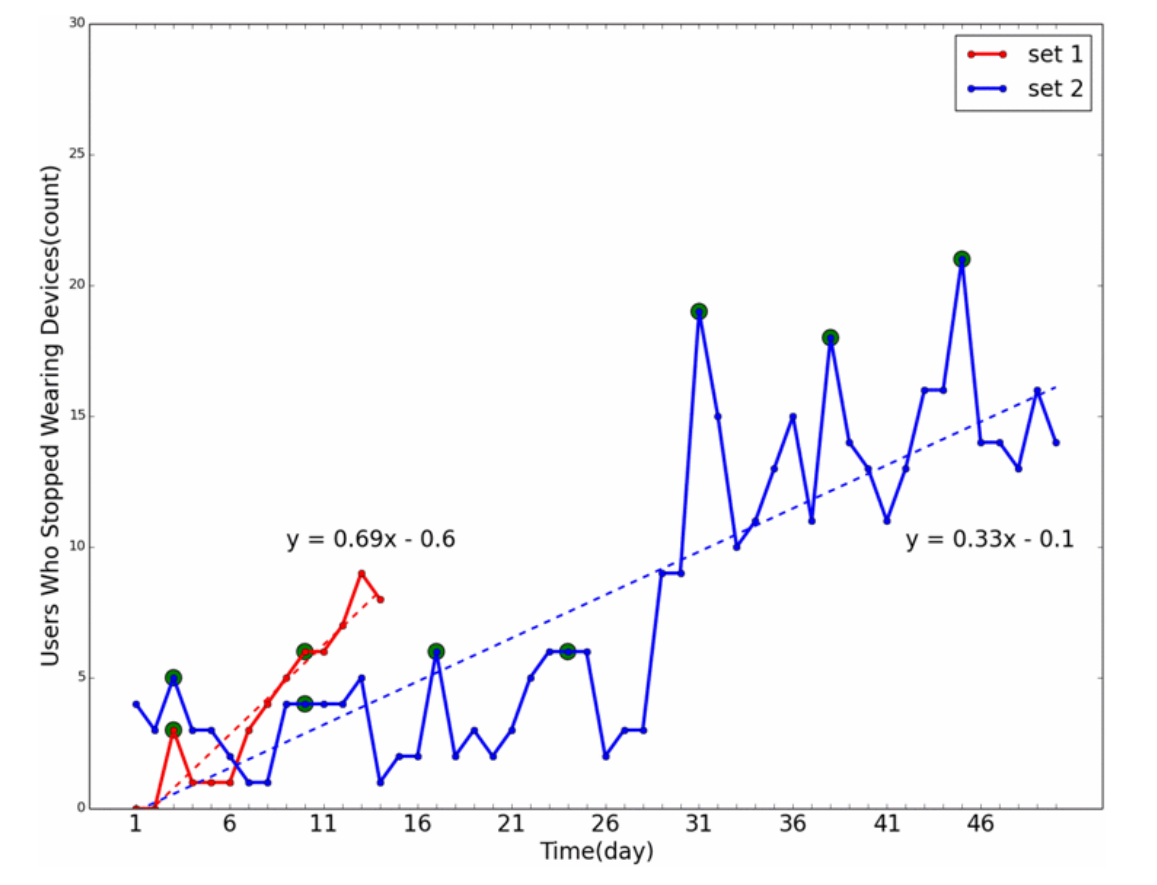
\includegraphics[scale=0.50]{figures/trackerAbandonment.png}
    \caption{Activity tracker abandonment rate \cite{Lee2017}}
    \label{acttrack}
\end{figure}

To try to deal with the problem of an inactive lifestyle and high abandonment rate of activity trackers and application, this project will develop a high-fidelity prototype with a focus on social cooperative fitness. The functionality from the prototype will log training data for friends, families or work place colleagues that have similar fitness goals in mind. The goal of the application is to encourage exercise and keep each member accountable of each other to promote physical health by achieving short-term and long-term goals.

\textbf{The hypothesis is that the social logging functionality would improve the accountability and motivation for using activity trackers and applications by letting users stay accountable of each other with small groups where they can log their workouts and having both short-term and long-term goals.}

The scientific approach will be design science which provides methods where relevant solutions will be designed for real people and environments with the goal of contributing to the existing knowledge base. Working with the user group, potential users have been interviewed and presented with different design choices and contributed with their information needs and preferences. 

\begin{figure}[H]
    \centering
    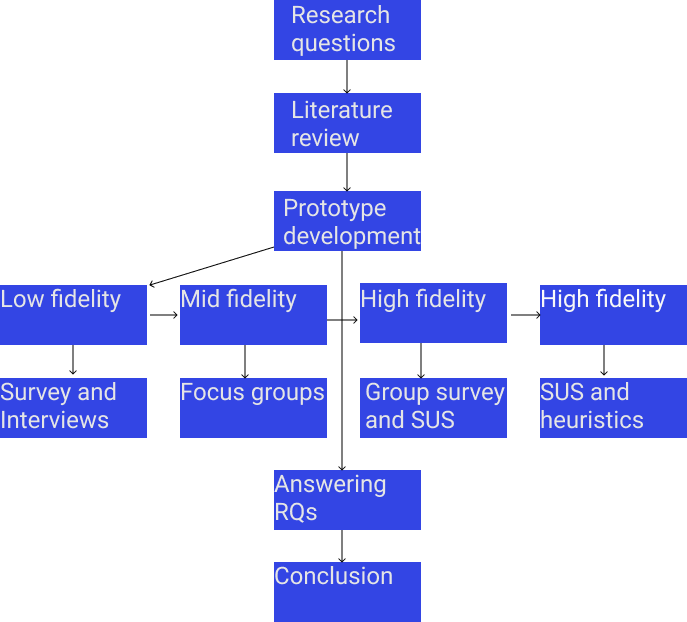
\includegraphics[scale=0.50]{figures/masterflowchart.png}
    \caption{The flow of the thesis, starting with the research questions. A literature review was done to show the dangers of a sedentary lifestyle and review the current research in human-computer interaction. The prototype development shows all the data gathered throughout this project from surveys,interviews, focus groups and user testing. The discussion answers the research questions and last is the conclusion.  }
\end{figure}

\section{Research Questions} \label{RQs}
\begin{enumerate}
    \item What functionality should be included in a social fitness application for users who struggle with a sedentary lifestyle, that would motivate them to improve their lifestyle? 

    \item Can the application functionality assist users in staying accountable for working out and logging their progress?
\end{enumerate}
\newpage
\subsection{Goals}
The goals of the research are:
\begin{enumerate}
\item Identify what social group features works for fitness applications
\item Present feature recommendations which can be used by established fitness applications
\item Develop a prototype for testing the features
\item Do development iterations, implement feedback
 and present potential improvements of the prototype functionality 
\end{enumerate}
The goals of the features are to get users to staying accountable to working out and logging their workouts and progress while cooperating with friends and families to meet their personal and group goals.
This thesis will contribute recommendations on how fitness applications should incorporate social features and functionality to keep the users engaged, motivated and accountable.
 
\newpage
 
\section{Outline of research project}
The following is the outline of the research project:

\textbf{Chapter 2: Sedentary lifestyle and benefits of exercise} Shows the dangers of sedentary lifestyle, explains exercise and strength training, looks at how people are motivated and benefits of exercise.

\textbf{Chapter 3: Literature review} Summarises the literature and related work for this project, relevant literature in human computer-interaction and computer supported cooperative work. References studies done with work colleagues, friends, how information is shared and the social incentives for fitness applications. Overview over fitness tracking and devices and the benefits of using them.

\textbf{Chapter 4: Methodologies} Explains the methodologies that are used in this project and the contributions

\textbf{Chapter 5: Requirements} Shows ethical considerations, the target group, participants of the project and the requirements that was gathered from the users

\textbf{Chapter 6: Prototype development} Shows the design iteration, the scientific process and summaries of each iteration from the user feedback

\textbf{Chapter 7: Features of application} Shows the high-fidelity prototype and the functionalities

\textbf{Chapter 8: Evaluation} Summarises the results from all the evaluations from this project

\textbf{Chapter 9: Discussion} Answers the research questions and the use of the different methodologies and the development process

\textbf{Chapter 10: Conclusion and future work} Concludes the project and recommendations for future work





\chapter{Sedentary lifestyle and exercise}
This chapter highlights what exercise and strength training is, how it can be done and the benefits of exercising. The chapter also looks at the different problems that can arise from living a sedentary lifestyle. What motivation is in terms of exercise, how users can be inspired and motivated.

\section{Benefits of exercise}
There are many benefits of working out and increasing your physical activity for health. As a sedentary lifestyle may lead to lifestyle diseases like cardiovascular problems and diabetes, staying active and in shape has benefits to everything from decreasing the chances of lifestyle diseases to improving mental health, sleep and cognition. Exercise has positive influences on cognitive abilities and sleep quality improves with exercise \cite{Lurati}. Workers, who are physically fit, usually have a low resting heart rate.

\section{Problems of sedentary lifestyle}
More problems
Besides the physical problems of being sedentary, there are other problems that are related to being inactive,people who has experiences with weight stigma were related to lower self-esteem, increased depression and increased body dissatisfaction \cite{Friedman}.
A person who lives a sedentary lifestyle might be afraid of going to the gym \cite{Vartanian2008}. Embarrassment caused by actual or anticipated negative evaluations from others might motivate some people to actively avoid public exercise situations, such as fitness centers and swimming pools. This is a common way of thinking where people are afraid of doing exercises the wrong way and are afraid that others will make fun of them. A way of eliminating this issue is to increase the knowledge among potential gym goers and people who live a sedentary lifestyle, encouraging them through technology to increase their own knowledge about exercise and physical fitness.

\section{Daily steps and cardiovascular health}
As regular physical activity is suggested as an important method to prevent cardiovascular diseases. There have been suggestions made that only walking is enough to stay physical fit and that people who walk 10000 steps a day has less chances of having cardiovascular risk factors. The correlation have been verified that people who walked more than 10000 steps a day had less body mass index, body fat percentage and triglycerides. Whereas the people who did not walk 10000 steps a day had greater chances of being overweight and dyslipemedia \cite{Rodrigues}. Thus concluding that there is an association between daily steps and cardiovascular risk factors. However it is not enough to remain physically fit as regular exercise is needed as well \cite{WHO}.

\section{Exercising and strength training}
A way of staying physically active is to exercise and do strength training, strength training is exercise that develops the strength and endurance of large muscle groups. It is also called “resistance training” or “weight training\cite{Resistance}. Strength training increases the fitness level, muscular strength, endurance, changes the body composition and more power. Even for frail elders it is understood that exercise and resistance training is positive. Supervised and controlled resistance training represents an effective intervention in frailty treatment \cite{Lopesz}.

By progressively overloading the weights that are lifted, or increasing repetitions or sets of exercises, people have a quantitative way of logging the progression. By setting short term or long-term goals like wanting to lift 100 kg in bench press makes it possible to both see progression, as you get stronger and stay motivated as you have a long-term goal.
if people want to stay active, motivated and encouraged it is good to get a partner. Exercising with a friend or relative can make it more fun. An exercise partner can offer support and encouragement \cite{FriendWorkout}. Exercising with friends and family will hold you accountable, Also, you will be less likely to skip a day of exercise if someone else is counting on you. And that when you work out, you should vary your routine. You are less likely to get bored or injured if you have some variety in your exercise routine. Keep track of your exercise to stay motivated. Use an app on your phone or a wearable activity tracker. You can even just mark a calendar with a checkmark each day you exercise \cite{FriendWorkout}.
\section{Motivation and exercise}
Motivation is a key feature of exercise and can account for individual differences in behaviours, inspiring people to engage in exercise \cite{Patel2015}.
Motivation for exercise can be divided into two categories, intrinsic motivation and extrinsic motivation. “Intrinsically motivated actions are experiences of competence, interest and enjoyment” \cite{Richard}, these are desires to engage new challenges and expand the skills.  “Extrinsic motivated behavior are those that are performed in order to obtain rewards or outcomes that are separate from the behavior itself” (ibid). These are body related motives, improving the appearance by losing weight or gaining more muscle, or fitness related motives like lifting more weight in the deadlift.  

A study done by Kilpatrick et al\cite{Kilpatrick} researched the motivation for physical activity for college students and reported that “results indicate that participants were more likely to report intrinsic motives, such as enjoyment and challenge, for engaging in sport,  whereas motivations for exercise were  more extrinsic and focused on appearance and weight and stress management. Since exercise has increasingly become a programmed activity \cite{Richard} they made the suggestion that making exercise or physical activity more intrinsically motivating(fun, personal challenging) might be a viable route to enhance persistence.” Another motivation for exercising is the increase in positive affect, the positive feelings about yourself, being able to relax and having increased energy, exercising gives the exerciser an enhanced sense of self in a pressure-free environment\cite{Frederick}.

\chapter{Literature Review}
This chapter is about the literature review for this project. In this chapter, the relevant literature and theories will be reviewed. The literature review will examine the dangers of an inactive lifestyle and the benefits of exercising and the existing tools and technologies that have been proposed to solve the issue Reviewing the current research in human-computer interaction that involves exercise and health. What research has been done with health and exercise tracking with colleagues in work places and friends. The chapter looks at the social incentives, competition, cooperation and social influence that comes from fitness application. It looks at gamification, what it is, and what effect leaderboards have on users.

\section{HCI and promoting physical activity}
Ahtinen et al\cite{Ahtinen2009} did a study on wellness and the effect of using ubiquitous technologies and mobile phones to see the social interaction and information sharing in groups that had similar fitness goals. They found that using communication technology to spread wellness-related information and applications as gifts within a network of trusted of people. This gives the initial motivation and push to start using wellness applications and working towards better wellbeing. They also suggested that having peer-support from people with similar goals can increase the motivation to reach a better wellness level. One of the interviewed participants in the study noted that maybe there could be some option of also uploading some new[exercise] combinations which you have discovered, and you want to share with other users.

Sharing a fitness goal and activities with friends can increase the motivation for users and impact the general health of those that share them publicly. Announcing  commitments can catalyze support and accountability from existing social networks for health behavior change \cite{Munson2015}. However, they found that announcing your public fitness goal creates a selection effect that decreases the probability of making commitments (ibid).  By having private groups consisting of friends and families instead of sharing your fitness goals on social media could increase the probability of participating and increase the follow-through.

A study by Chen et al\cite{Chen2017} looked at the effect of using a leaderboard as a social incentive to track fitness data and researched the difference in interaction between workplace colleagues and chronically ill. The research showed that both groups were motivated by having a leaderboard for their fitness tracking. The healthy groups of participants saw the leaderboard as a competition whereas the chronically ill groups used it as a way of obtaining information from other patients. 

\section{Health tracking in work places}
Many companies have health incentives for their employees where they can get gym membership discounts and even monetary incentives as motivation for reaching a goal. A study by Chung et al\cite{Chung2017} researched the health tracking in work places that had wellness programs for their employees. The study suggests that sharing fitness data between the employees supported the fitness tracking. Having a collective goal such as walking 7000 steps every day was also beneficial to the fitness tracking.  individuals participating in team-based step-counting initiatives become accountable to each other for both the number of the steps they take and their reasons for walking. \cite{Buis2009}

A study done by Xipei et al\cite{Ren2018} explored this further to see if cooperative fitness tracking in work places encouraged physical activity. The study had participants that were divided in to groups of two and each group had a collective goal for daily steps. The study found that the participants were more active compared to the initial baseline week. The participants that were in the same office or proximity of each other did more physical activity than the participants that were in different offices. In addition, the participants that were closer would communicate more with each other and share information and knowledge of workouts. 

\section{Social incentives for fitness applications}
A paper by Chen and Pu\cite{Chen2017} looked at social incentives for mobile fitness applications where they developed a mobile game to understand how users interact in groups for competition or cooperation. The participants increased their physical activity significantly when paired up in the groups, however they found that “competition motivates dyads if they have equivalent performances and availabilities, but is likely to demotivate them if otherwise”\cite{Chen2017}. A better social incentive for a fitness application if the groups have different levels of performance is for them to cooperate with each other instead of competing.  “Cooperation setting is more likely to stimulate users to interact with each other via messages than competition settings”(ibid), having the users cooperate increases the interaction and possibly the knowledge sharing in between them.

Another social incentive is social influence, which consists of social comparison and social support.” In fitness apps, using leaderboards, people could easily check their relative performance positions”\cite{Zhou2018} for comparing themselves in social networks, and receiving social support by receiving positive feedback and comments.

Using cooperation as a social incentive, it is better to use strong ties consisting of friends, families or colleagues than strangers with weak ties. “Participants found community competition and the support from strong ties motivating, however, pairing up with weak ties was reported demotivating”\cite{Chen2016} Also suggesting that by creating a community effect for the competition will increase the cooperation and maybe have mentors that share knowledge.

\section{Gamification and fitness applications}
Gamification in fitness applications refers to the “the use of game design elements in nongame contexts” \cite{Deterding}. It is a popular strategy as a way of motivating users to adopt and use their application. A way of gamifying fitness applications may refer to the use of augmented reality where the users can run routes and pick up objects in the game, or just having an overall leaderboard for the people that have worked out the most in a period.

 “Gamification may be an effective means of targeting motivational components, and games may be effective at triggering individuals and increasing popularity of apps”\cite{Lister} and “external incentives are enough to sustain (health) behavior responses without using other components of games like problem solving, storytelling, and fantasy”(ibid).  For long term health change and motivation, the external incentives are enough, the study shows there is no need for augmented reality, 3d technology or storytelling.  The same study shows that gamification mostly works for easy physical activity like walking, “complex behaviors such as diet and physical activity”(ibid), which may lead to more knowledge and a better long term health change for the users.

\section{Comparison, competition and cooperation in fitness applications}
 Social support and social pressure positively influence user motivation\cite{Buis2009}, most fitness applications have features where the users are able to either compare, compete or cooperate with other users. Comparison in fitness applications is defined as “the design that facilitates benchmarking individual’s fitness performance with that of others, and hence provide an opportunity for enhanced motivation in target behaviors” \cite{Yoganathan2013}. The users can compare their own results with others, for example compare how much time spent doing a given task. Another popular feature is competition, which in fitness applications is “the design that motivate enhanced physical activity performance by leveraging human’s natural drive to compete” (ibid). This is usually done with a leaderboard where users are ranked on how much they have worked out or their time or how many steps they have done within a timeframe.  Lastly there is cooperation in fitness applications is “the design that motivates users to adopt physical activity behavior by leveraging an individual’s natural drive to cooperate” (ibid). Users can cooperate and work for a common goal, share information and knowledge and form social bonds with each other.

 

\section{Fitness tracking and devices}
People track their fitness activity in diary reports and blogs.\cite{Goodman} Tracking your activity is beneficial for fitness behaviour change \cite{mccormick2015psychological}, logging workouts to show the progress in terms of weights lifted as well as tracking other goals like losing or gaining weight helps the overall behaviour change. Many mobile fitness applications design revolves around tracking activity and goal setting where the aim is to increase the users physical activity \cite{consolvo2007conducting}. 
The majority of HCI research that investigates fitness
technology use and tracking is for the purpose of evaluating specific fitness technologies\cite{Patel2015}. 

People that use devices and fitness trackers often abandon devices because they do not fit with their conceptions of themselves, the data collected by the devices are perceived to not be useful, and device maintenance became unmanageable. \cite{Lazar2015}. Unless the goal of a person is to track their steps and activity, devices purchased often do not appear to map to goals\cite{Lazar2015}. Goals like becoming a better table tennis player, or obtaining knowledge from others. People perceive the data collected as not useful because they are not interested in the level of information the data gives them. Many people mention that the number of steps they take is not interesting\cite{Lazar2015}. 

The ability for users to set their own primary and secondary goals is key for technology-based health interventions to be successful\cite{inproceedings}

\section{Related work}
There are several applications within the area of fitness and exercise. The applications allow users to obtain information and workouts, track their food consumption and daily exercise and even get personalized templates from personal trainers or buy training programs from fitness influencers. Some of the similar applications are:
Fitbit: “Without a tracker, the Fitbit app can count your steps (provided your carry your phone all day long), help you track the calories you consume, log your weight, and record other health information, such as blood pressure and glucose levels. If you do own a Fitbit tracker, the app is even easier to use because it logs a good amount of information about your activity automatically.”\cite{Duffy}
FitStar: “FitStar creates custom workouts for you based on your fitness level. You start by doing a few workouts with the app and you give it feedback as you go about which exercises were too tough, too easy, or just right. The app uses that information to create a routine that challenges you in all the right ways.”(ibid)
Lose it: “The free website and app Lose It!, designed for counting calories and logging exercise, can help you lose weight, especially if you tend to eat name-brand American foods. Lose It!, which has been around for years, has an incredibly strong community of supportive people to help you stick to your goals.”(ibid)
MyFitnessPal:” MyFitnessPal is a mobile app and website that gives you a wealth of tools for tracking what and how much you eat, and how many calories you burn through activity”(ibid)
Google Fit:” it's extremely serviceable and it's one of the better free fitness apps. It can do a lot of stuff. You can track your fitness using a point system as well as active minutes. The app also features fitness goal tracking, customized tips, and integration with a variety of other apps like Runkeeper, Strava, MyFitnessPal, and others. \cite{Hindy}
Gravitus: “Gravitus is the app for weight lifters. We live in a digital world and yet lifting is done completely offline. We're building the future of lifting. Enter the gym knowing exactly what you need to do. Record your workouts with a tool designed for speed. Celebrate your progress and break through plateaus. And connect with friends and others to stay motivated. Gravitus helps you reach your goals at the gym and have more fun doing it.”\cite{Gravitus}


\chapter{Methodologies}
This chapter is about the material and research methods that will be used for this project. The methodologies are important in research to help with the design and evaluation of the project. 
\section{Design Science}
“Design science research is a method that establishes and operationalizes research when the desired goal is an artefact or a recommendation” \cite{Dresch}. It includes users, the developers and research experts of various backgrounds.
Figure \ref{fig:Hevner2007} refers to the environment in which the artefact is observed, the environment is the people, the organizations and the technology. Design science research supports the development of the artefact that solves a problem and the goal is to increase the existing knowledge base. The artefact is evaluated and justified and the knowledge base can be used for the existing foundations and methods that are recognized by the scientific community.

The relevance cycle goes from requirements and field testing to the design cycle and rigor cycle and then adds to the knowledge base.
\begin{figure}[H]
    \centering
    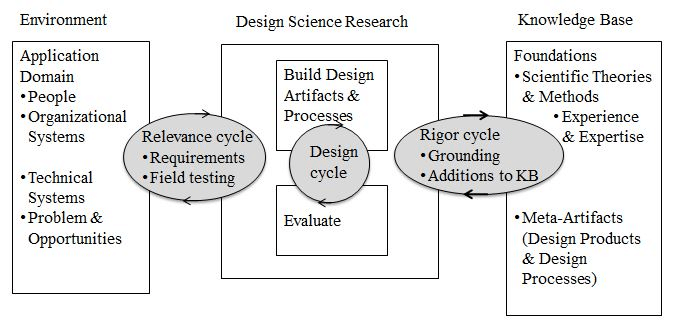
\includegraphics[width=120mm]{figures/Design-Science-Research-Cycles-Hevner-2007.png}
    \caption{Design science in information science research \cite{Hevner2007}}
    \label{fig:Hevner2007}
\end{figure}

Hevner et al \cite{Hevner2004} lists seven criteria that are essential for design research. The first criteria is the creation of a new artefact that has to solve a specific problem. The utility of the artefact has to be explained and later evaluated. The contribution of the artefact has to be clarified for academics and professionals interested in solving problems to increase the knowledge of the area. The validity of the artefact has to be rigorously tested and demonstrated to show that the artefact is suitable for the proposed use. The researchers have to understand the problem, and the results should be communicated in a proper way to those that are interested in the area.

Hevner and Chatterjee suggests a checklist for researchers to ensure that all the key aspects of design science research are being covered \cite{Hevner2010}. The questions from the checklist can be seen on page \pageref{tab:1} . Design science includes the users, developers and experts with a variety of backgrounds. With documentation about the research process it is possible to get a good development process with relevant results to the research.

\newpage
\begin{table}[H]
\begin{tabular}{ |l|l| }
  \hline
  \multicolumn{2}{|c|}{Questions} \\
  \hline
1 & What is the research question (design requirements)?\\ 
\hline
2 & What is the artifact? How is the artifact represented?\\
\hline
3 & What design processes (search heuristics) will be used to build the artifact?\\ 
\hline
4 &\makecell[l]{ How are the artifact and the design processes grounded by the knowledge base? \\What, if any, theories support the artifact design and the design process?} \\
\hline
5 &\makecell[l]{ Which evaluations are performed during the internal design cycles?\\ Which design improvements are identified during each design cycle?}\\ 
\hline
6 & \makecell[l]{How is the artifact introduced into the application environment and how is it field tested?\\ What metrics are used to demonstrate artifact utility and improvement over previous artifacts?}\\ 
\hline
7 &\makecell[l]{ What new knowledge is added to the knowledge base and in what form \\ (e.g., peer-reviewed literature, meta-artifacts, new theory, new method)?}\\ 
\hline
8 & Has the research question been satisfactorily addressed?\\
 \hline
  
\end{tabular}
\label{tab:1}
\caption{A checklist for researchers, key aspects of design science research}
\end{table}

\section{Conceptual Design}
Conceptual design uses the established requirements for the application and transforms it into a conceptual model\cite{interactiondesignbook}, the model shows the main functionalities of the application and lets the users interact with it. The key principles of conceptual design is to have an open mind, but not forget the users and their context. To discuss the ideas with other stakeholders. Use prototyping to get rapid feedback and do many iterations \cite{interactiondesignbook}. A conceptual model is very beneficial in the beginning phase of development.
\section{Prototyping}
Prototypes are a simplified version of an artefact design that are created with the purpose to test design features. “Prototyping is a key activity within the design of interactive systems” \cite{Buchenau}. Users are able to test and evaluate functionalities of the system before the artefact is finished and give feedback.  The evaluation and feedback from the prototype testing will lead to improvements of the prototype. Prototypes are divided between levels of fidelity, ranging from low-fidelity to high-fidelity. This research project will use three different levels of fidelity for the prototyping.

Low-fidelity prototyping \cite{interactiondesignbook} can be used to create a layout and test different design options. Low-fidelity prototyping includes three different methods that will be used in to project.

1. Sketching, cheap and time effective way of testing different design options, drawn by hand.

2. Wireframing, represents the layout and the content.

3. Mock-up, displays how the design looks with colours, content and in-depth descriptions.

Mid-fidelity prototyping is a mixture between the correct content and some functionality.

High-fidelity prototyping is closer to the end product of the application. With this prototype it is easier to do usability evaluation and let users test the functionalities and look at the content-

\section{Design Principles}
Design principles \cite{DesignP} are guidelines and design considerations which interaction designers focuses on for the user experience and user interface of a product. There are five principles that are important to consider while integrating features for an interface.

Visibility is the first principle that states that the more visible an item is, the more likely a user will know it and use it. \cite{Norman} The user interface should be intuitive.

Feedback is the principle of making it clear what action has been taken and what has been accomplished \cite{Norman}. The user should not have to guess what their action accomplished and there should be feedback in the form of visual, tactile or audio.

Constraints is about limiting the range of interaction possibilities for the user to simplify the interface and guide the user to the appropriate next action \cite{Norman}. Constraints makes it harder for a user to make mistakes.

Consistency refers to having similar operations and similar elements for achieving similar tasks \cite{Norman}. The design should not have any surprises.

Affordance refers to an attribute of an object that allows people to know how to use it \cite{Norman}, by using symbols that users are accustomed to, they will already understand what the action is. 


\section{Data Gathering}
This chapter covers the evaluation methods that will be used for this project. The evaluation methods are important for the research rigor and design research process to demonstrate the utility, quality and efficacy of the artefact.
Quantitative methods are focused on gathering large quantities of data and is collected through polls, questionnaires, surveys and more. The data can be used for statistical analysis.
The qualitative research in this project will be based on semi-structured interviews, observations and focus groups. Qualitative research focuses more on in-depth research and fewer data collection cases.

\subsection{Literature Review}
A literature review is gathering of published articles, reports, books and other relevant documents by searching with keywords in academic journals and search engines. The literature review shows a summary of relevant information about methods, data gathering and what the research accomplished. The literature review can contribute to finding and establishing requirements for the artefact development.

\subsection{Semi-Structured Interview}
Semi-structured interviews uses pre-defined questions to create a structure of an interview. The prepared questions are asked and are open for answers and discussions. The method allows for follow up questions and exploring discussions. This method was used during the interviews with ... An interview guide approved by NSD can be found in appendix ..

\subsection{Survey}
A survey is a quantitative method of gathering data with the purpose to produce statistics about some aspects of a sample population. A survey collects information by asking people questions and the answers are the data that is analyzed \cite{fowler2013survey}. The questions are mainly close-ended with few open-ended questions at the end for free form answers.
\subsection{Focus Groups}
A focus group is a group interview with several participants at the same time with a moderator present to ask questions and guide the conversation. “Focus groups explicitly use group interaction as part of the method. This means that instead of the researcher asking each person to respond to a question in turn, people are encouraged to talk to one another: asking questions, exchanging anecdotes and commenting on each other's experiences and points of view”\cite{Kitzinger}. The experiences and points of view can be used to identify common knowledge and get feedback in a setting that is more relaxed than in a laboratory. The focus group will consist of many members. 

\subsection{Case Study}
A case study is an intensive study about a person, a group of people or a unit where the aim is to generalize over several units \cite{Heale7}. In this project, a group of people were asked to explain how they log their workouts and how they would interact with the application.
\section{Evaluation of Prototypes}
Evaluating a prototype is part of the developmental phase and is performed at the end of each iteration. There are different ways of evaluating a prototype. Experts and users can be included to be certain that the prototype is relevant and the design is easy to use, easy to learn and the design is intuitive. 

\subsection{Usability Testing}
Usability testing is testing a prototype with participants that represent real users \cite{dumas1999practical} . The users play around with the prototype and perform real tasks while their actions are observed and notes are taken. The goal of a usability test is to improve the usability of a product, analyse data and find problems and reiterate the development phase to improve the prototype.
\subsection{System Usability Scale}
Another way of evaluating HCI is to use the system usability scale by John Brooke \cite{Brooke}. This evaluation method differs from the heuristic evaluation by having regular users that are not experts in the field of HCI to evaluate the system. The system usability scale consists of ten statements, every statement gets a score where strongly disagree is the weakest and strongly agree is the strongest.
The SUS score can be calculated and there are different ways of measuring it, grades, adjectives or percentages can be used \cite{doi:10.1080/10447318.2018.1455307} . The ten statements are structured so that odd numbers have positive loaded questions and even numbers have negative loaded questions. To calculate the score, the odd numbers will have 1 subtracted from their value and the even numbers will subtract their number from the value 5. Adding this together and then multiplying it with 2.5 will get a SUS score out of 100. A SUS score above 68 is considered as a good score \cite{doi:10.1080/10447318.2018.1455307}. 
\begin{figure}[H]
    \centering
    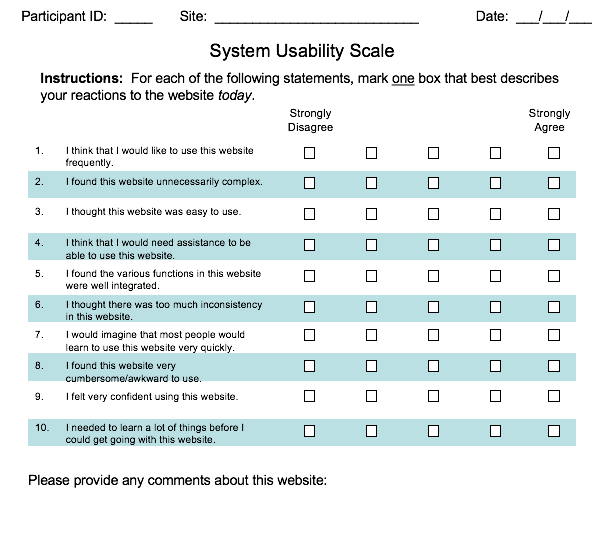
\includegraphics[width=120mm]{figures/sus-template.png}
    \caption{System usability scale template}
\end{figure}


\subsection{Nielsen`s Heuristics}
To evaluate the usability of a system, Nielsen \cite{Nngroup} developed ten heuristics as a guideline to test and estimate the usability of a product. The ten heuristics can be used by human computer interaction experts to evaluate the interface of an application. The evaluation is performed by a small set of usability experts individually and only requires a few experts to identify 75\% of the problems \ref{NN}.

\begin{figure}[H]
    \centering
    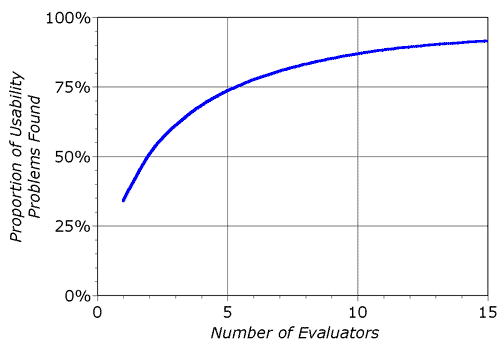
\includegraphics[width=120mm,height=8cm,keepaspectratio]{figures/heur_eval_finding_curve.png}
    \caption{The proportion of usability problems in an interface using various numbers of evaluators\cite{Nngroup}}
    \label{NN}
\end{figure}
Nielsen`s heuristics will be tested by experts in information science.

\begin{table}[H]
\hskip-1.5cm\begin{tabular}{ |l|l| }
  \hline
  \multicolumn{2}{|c|}{Nielsen`s Heuristics} \\
  \hline
\makecell[l]{Visibility of system\\ status} &\makecell[l]{The system should always keep users informed about what is going on,\\ through appropriate feedback within a reasonable time.}\\ 
\hline
\makecell[l]{Match between the\\ system and the real world} &\makecell[l]{ The system should speak the users' language, with words, phrases, and\\ concepts familiar to the user, rather than system-oriented terms. Follow\\ real-world conventions, making information appear in a natural and\\ logical order.}\\
\hline
\makecell[l]{User control and\\ freedom} & \makecell[l]{Users often choose system functions by mistake and will need a clearly\\ marked "emergency exit" to leave the unwanted state without having to\\ go through an extended dialogue. Support undo and redo.}\\ 
\hline
\makecell[l]{Consistency and\\standards}  & \makecell[l]{Users should not have to wonder whether different words, situations,\\ or actions mean the same thing. Follow platform conventions.} \\
\hline
\makecell[l]{Error prevention} & \makecell[l]{Even better than good error messages are a careful design which prevents\\ a problem from occurring in the first place. Either eliminate error-prone\\ conditions or check for them and present users with a confirmation option\\ before they commit to the action.}\\ 
\hline
\makecell[l]{Recognition rather than\\ recall} & \makecell[l]{Minimize the user's memory load by making objects, actions, and options\\ visible. The user should not have to remember information from one part\\ of the dialogue to another. Instructions for use of the system should be\\ visible or easily retrievable whenever appropriate.}\\ 
\hline
\makecell[l]{Flexibility and\\ efficiency of use} & \makecell[l]{Accelerators — unseen by the novice user — may often speed up the\\ interaction for the expert user such that the system can cater to both\\ inexperienced and experienced users. Allow users to tailor \\frequent actions.}\\ 
\hline
\makecell[l]{Aesthetic and\\ minimalist design} & \makecell[l]{Dialogues should not contain information which is irrelevant or rarely\\ needed. Every extra unit of information in a dialogue competes with\\ the relevant units of information and diminishes their relative visibility.}\\
\hline
\makecell[l]{Help users recognize,\\ diagnose, and recover\\ from errors} &\makecell[l]{Error messages should be expressed in plain language (no codes),\\ precisely indicate the problem, and constructively suggest a solution.}\\
\hline
\makecell[l]{Help and documentation}&\makecell[l]{Even though it is better if the system can be used without documentation,\\ it may be necessary to provide help and documentation. Any such\\ information should be easy to search, focused on the user's task,\\ list concrete steps to be carried out, and not be too large.}\\
  \hline
  
\end{tabular}
\label{tab:2}
\caption{Nielsen`s heuristics to follow for user interface}
\end{table}



\newpage

\subsection{Obervations}
Another qualitative method to evaluate an application is observations. “Individuals are observed performing specified tasks within a controlled environment”\cite{Preece}. The evaluator has a script and predetermined tasks for the participants. They are encouraged to communicate while they are performing the tasks and use the think-aloud technique which is a technique developed by Erickson and Simon\cite{Erickson2}. The technique requires the participants to say out loud what they are thinking and trying to do. Thus making it easier for the evaluator to take notes, which can be analyzed later.


\chapter{Requirements}
This chapter includes the ethical considerations for the project and the appropriate approvals that was secured from the Norwegian Centre for Research Data. The chapter presents the target group, the users that participated in testing the project, the experts... The requirements that were gathered from analysing stuff
\section{Ethical Considerations}
All participants were informed of their rights to be removed from the research project at any time and that their privacy is respected and secured. The participants were not asked any sensitive questions about their private life. 

The research was approved by the Norwegian Centre for Research Data (Norsk Senter for Forskningsdata - NSD). The participants signed an inform consent before being interviewed, testing or evaluating. The approval from NSD can be found in appendix .. Inform consent and interview guides can be found in appendix ..
\section{Target Group}
The target group is young adults between the ages of 18-30, who lives a sedentary lifestyle or exercise rarely and want to change. This was to focus on potential users who want to make adjustments and improve to maintain an active and healthy lifestyle. For the research it is important that the target group were interested in technology and were willing to use new applications. 

\begin{table}[H]
\centering
\begin{tabular}{ |l|l| }
  \hline
  \multicolumn{2}{|c|}{Target group} \\
  \hline
Gender & male/female\\ 
\hline
Age & 18-50\\
\hline
IT Criteria & smartphone, active on social media\\ 
  \hline
\end{tabular}
\label{tab:3}
\caption{Target group requirements}
\end{table}


\section{Research Participants}
\subsection{Users}
The users were recruited through personal connections. The users in the focus group which consisted of  one female and three males. Two of the users work in banking and investment, one masters student and one consultant. The focus group members averages one to two workout a week. 
The users in the case study and usability testing were two females, both are business and economics students and usually workout once or twice a week.
\subsection{Physical exercise experts}
The physical exercise experts consisted of a researcher in physiotherapy, a personal trainer and a former personal trainer who works as a developer. They were recruited through personal connections and took part in semi-structured interviews.
\subsection{Usability experts}
Six usability experts from the University of Bergen were recruited to evaluate the application with  Nielsen`s heuristics or SUS. The experts were one female and five males. The usability experts are all information science master students. The usability experts have a varied workout background, from being professional athletes that workout five to six times a week to living a sedentary lifestyle with no workouts. 
\section{Requirements}\label{requirements}
To establish requirements it is important to know who the users are, what features to implement and how to implement them. The requirements for a system are descriptions of services that a system should provide and constraints on its operation \cite{Sommerville:2010:SE:1841764}. The requirements are the needs of the features and are often divided in to functional requirements and non-functional requirements.
\subsection{Functional Requirements}
Functional requirements are the statements of services the system should provide, how the system should react to particular inputs, and how the system should behave in particular situations \cite{Sommerville:2010:SE:1841764}.
For the functional requirements it is important to understand what the user needs from the application. A survey on social media was conducted for the purpose of analysing what features users need.  

\textbf{The application needs to}
\begin{itemize}
\item store information the users want to share
\item let users select goals
\item display common goals for the groups
\item compete and cooperate towards goals
\item be able to see their own progress and group members progress
\item log workouts

\end{itemize}
    
\subsection{Non-Functional Requirements}
The non-functional requirements are the constraints on the services or functions offered by the system. The non-functional requirements include timing constraints, constraints on the development process and constraints imposed by standards \cite{Sommerville:2010:SE:1841764} . These requirements apply to the system as a whole rather than individual features. 

\textbf{The interface needs to}
\begin{itemize}
\item be user-friendly (fast responding, lean design)
\item be responsive
\item be aesthetically pleasing with modern design
\item be designed within the delivery of this paper(1st june 2020)
\end{itemize}
    
\chapter{Prototype Development}
\section{Iteration overview}
This chapter presents four design iterations and methods that were used while prototyping. The table below summaries the iterations and shows what methods were used and how the prototype was evaluated.
{
\begin{table}[H]
\centering
\hskip-1.5cm\begin{tabular}{ |l|l|l|l|l| }
  \hline
  \multicolumn{5}{|c|}{Overview of iterations} \\
  \hline
\makecell[l]{Iteration} &\makecell[l]{1}
&\makecell[l]{2}
&\makecell[l]{3}
&\makecell[l]{4}\\ 
\hline
\makecell[l]{Define/Redefine} &\makecell[l]{Literature review\\ and survey}
&\makecell[l]{Redefine after\\ expert interview}
&\makecell[l]{Redefine after\\ focus group}
&\makecell[l]{Redefine after\\ SUS with experts}
\\ 
\hline
\makecell[l]{Fidelity} &\makecell[l]{Low}
&\makecell[l]{Low-mid}
&\makecell[l]{High}
&\makecell[l]{High}
\\ 
\hline
\makecell[l]{Method} &\makecell[l]{Interview with\\ experts}
&\makecell[l]{Focus group \\ design principles}
&\makecell[l]{Group survey}
&\makecell[l]{SUS with experts}\\ 
\hline
\makecell[l]{Evaluate} &\makecell[l]{Evaluate with \\ experts}
&\makecell[l]{Interview}
&\makecell[l]{SUS with experts}
&\makecell[l]{SUS with users \\heuristics with\\ experts}
\\ 
\hline
\end{tabular}
\label{Overview}
\caption{Overview of design iterations}
\end{table}
}


\section{First Iteration of Research Project}
The first design iteration started with the requirements established from the literature review and a survey conducted through social media to gather data. The survey went through two pilot studies to establish the best way to get data and was shared on Facebook. The purpose of the survey was explained in the introduction, so that the people who answered knew what they were contributing to. They were shown an example of logging exercises \ref{fig:workout log} and were explained how a likert scale works. 44 people answered the survey.
\begin{figure}[H]
    \centering
    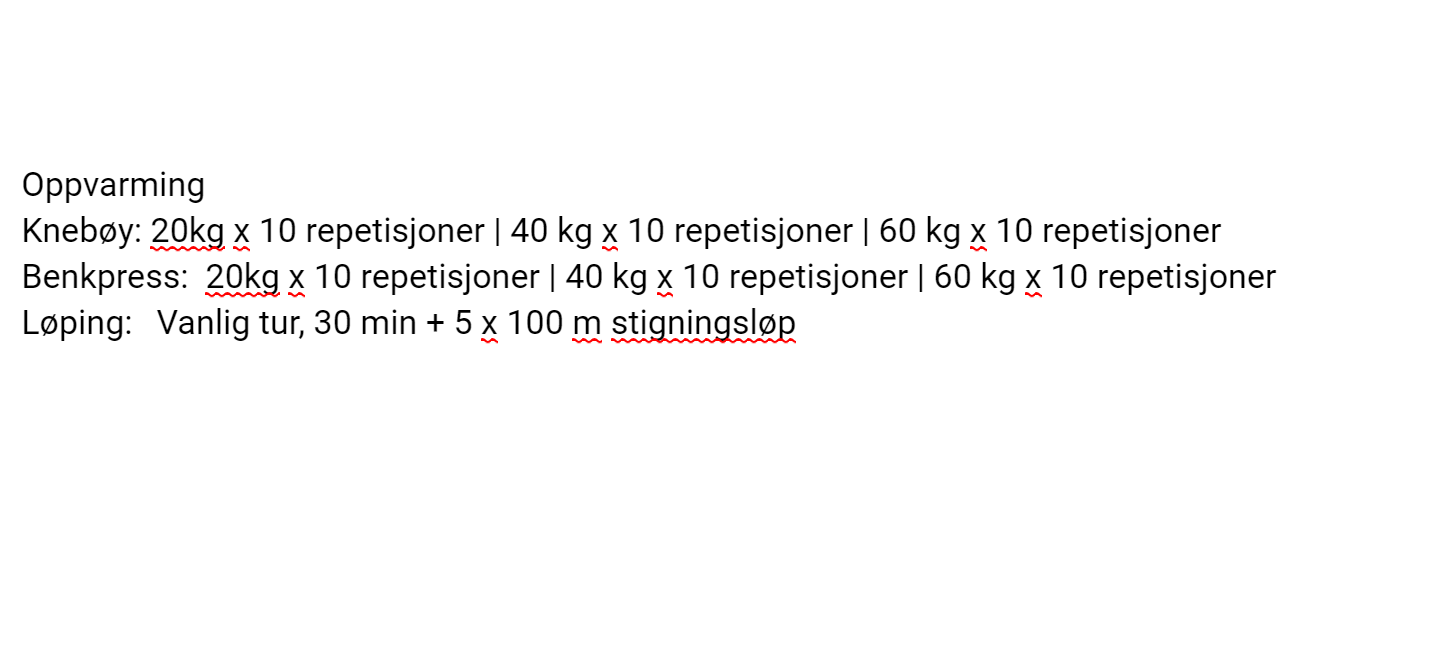
\includegraphics[width=120mm]{figures/testtest.png}
    \caption{Example of logging a workout}
    \label{fig:workout log}
\end{figure}
\subsection{The survey}
To establish some background information on the people that were surveyed, they were asked how often they work out and whether or not they already use an activity tracker. The majority of people that answered worked out more than 10 times a month and less than 30\% answered 5 or less.
\begin{figure}[H]%
    \centering
    {{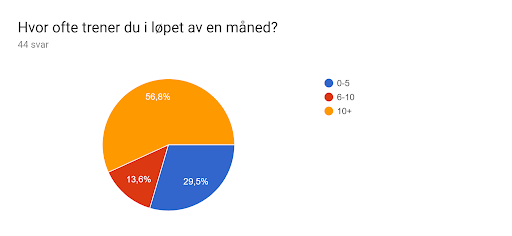
\includegraphics[width=7cm]{figures/testings.png} }}%
    \qquad
     {{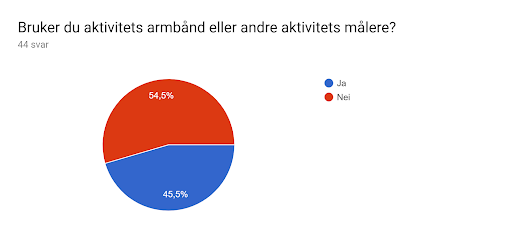
\includegraphics[width=7cm]{figures/survey2.png} }}%
    \caption{Background information}%
\end{figure}
45.5\% answered that they use an activity tracker and they were also asked to list which tracker they used which can be seen in the table below. 

\begin{table}[H]
\centering
\begin{tabular}{ |l|l| }
  \hline
  \multicolumn{2}{|c|}{Activity Tracker} \\
  \hline
Apple Watch & 2\\ 
\hline
Fenix & 1\\
\hline
Fitbit & 5\\ 
  \hline
  Garmin & 5 \\ 
  \hline
  Kadens & 1\\ 
  \hline
   Polar & 3\\ 
  \hline
   Suunto & 2\\ 
  \hline
\end{tabular}
\label{tab:3}
\caption{Survey Activity Tracker}
\end{table}

They were asked to list what kind of data they think is interesting besides logging workouts from the activity trackers and applications. Some of the answers are shown in the table below. Most people answered that knowing the heart rate, average heart rate and max heart rate is important. Also the amount of daily steps, distance of a run, amount of sleep and performance analysis were listed. 
\begin{table}[H]
\begin{tabular}{ |l|l| }
  \hline
  \multicolumn{2}{|c|}{Data from activity tracker} \\
  \hline
\makecell[l]{Norwegian} & \makecell[l]{English translation}\\ 
\hline
\makecell[l]{Distanse løpt/gått} & \makecell[l]{Distance run/walked}\\
\hline
\makecell[l]{Puls, tid og hastighet} & \makecell[l]{Heart rate, time and speed}\\ 
  \hline
\makecell[l]{Puls} & \makecell[l]{Heart rate} \\ 
  \hline
 \makecell[l]{Følge med om økten holder seg innenfor\\ mål satt før trening} & \makecell[l]{If the workout stays within the\\ pre-deterimined limits}\\ 
  \hline
  \makecell[l]{Puls, søvn, søvnforstyrrelse/urolig søvn,\\ skritt, kalorier, stigning/høydemeter} &
  \makecell[l]{Heart rate,sleep, sleep disturbances, steps,\\ calories, climb/ascent/acclivity}\\ 
  \hline
   \makecell[l]{Puls, løpedistase og tid} & \makecell[l]{Heart rate,distance run and time}\\ 
  \hline
   \makecell[l]{Skritteller,søvn og trenings analyse} &\makecell[l]{ Steps, distance, sleep and workout analysis}\\ 
  \hline
   \makecell[l]{Antall skritt gått} & \makecell[l]{Daily steps}\\ 
  \hline
   \makecell[l]{Performance, energiforbruk, treningseffekt og\\ restitusjonstid} & \makecell[l]{Performance, energy spent,\\ training effect, recovery time}\\ 
  \hline
   \makecell[l]{Gjennomsnittspuls} & \makecell[l]{Average heart rate}\\ 
  \hline
   \makecell[l]{Makspuls} & \makecell[l]{Max heart rate}\\ 
  \hline
\end{tabular}
\label{table:ActivityTrackerData}
\caption{Data from activity trackers}
\end{table}



To get more knowledge about the surveyed people`s workout habits, they were asked if they logged their workouts seen in figure \ref{workoutlogging}. The majority answered they do not log their workouts.  From the 41.9 \% of people that log their workouts were asked if they do it after or during and 70\% of them do it after they are finished with the workout.

\begin{figure}[H]
    \centering
    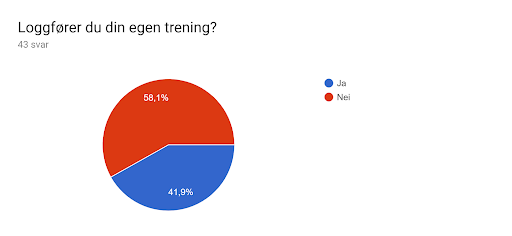
\includegraphics[width=120mm]{figures/loggforerduegentrening.png}
    \caption{Workout logging}
    \label{workoutlogging}
\end{figure}
To get an understanding of how people view others progress \ref{others}. They were asked if they feel extra motivated to workout by seeing friend`s progress, whether its strength progression or physical changes. 20 people answered that they agree or strongly agree. 13 answered neutral and 11 in total answered that they disagreed or strongly disagreed.
\begin{figure}[H]
    \centering
    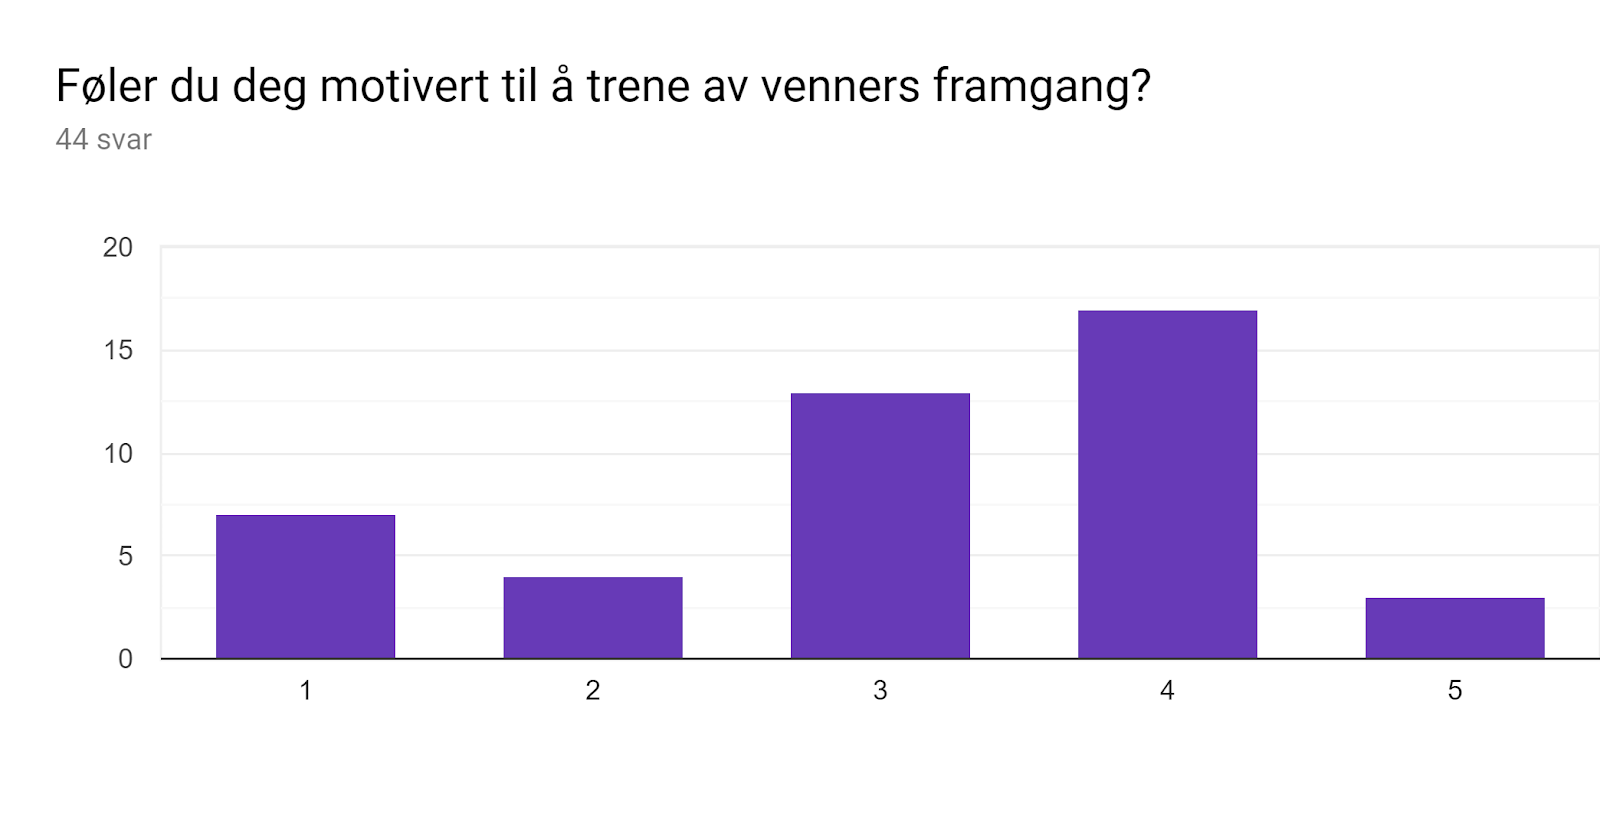
\includegraphics[width=120mm]{figures/MotivertAvAndresTrening.png}
    \caption{Motivated from others progress}
    \label{others}
\end{figure}
Since most people do not log their workouts, it is interesting to know if they would feel motivated to log their workouts if their friends could see the workout logs. However most people strongly disagree with this statement. 

\begin{figure}[H]
    \centering
    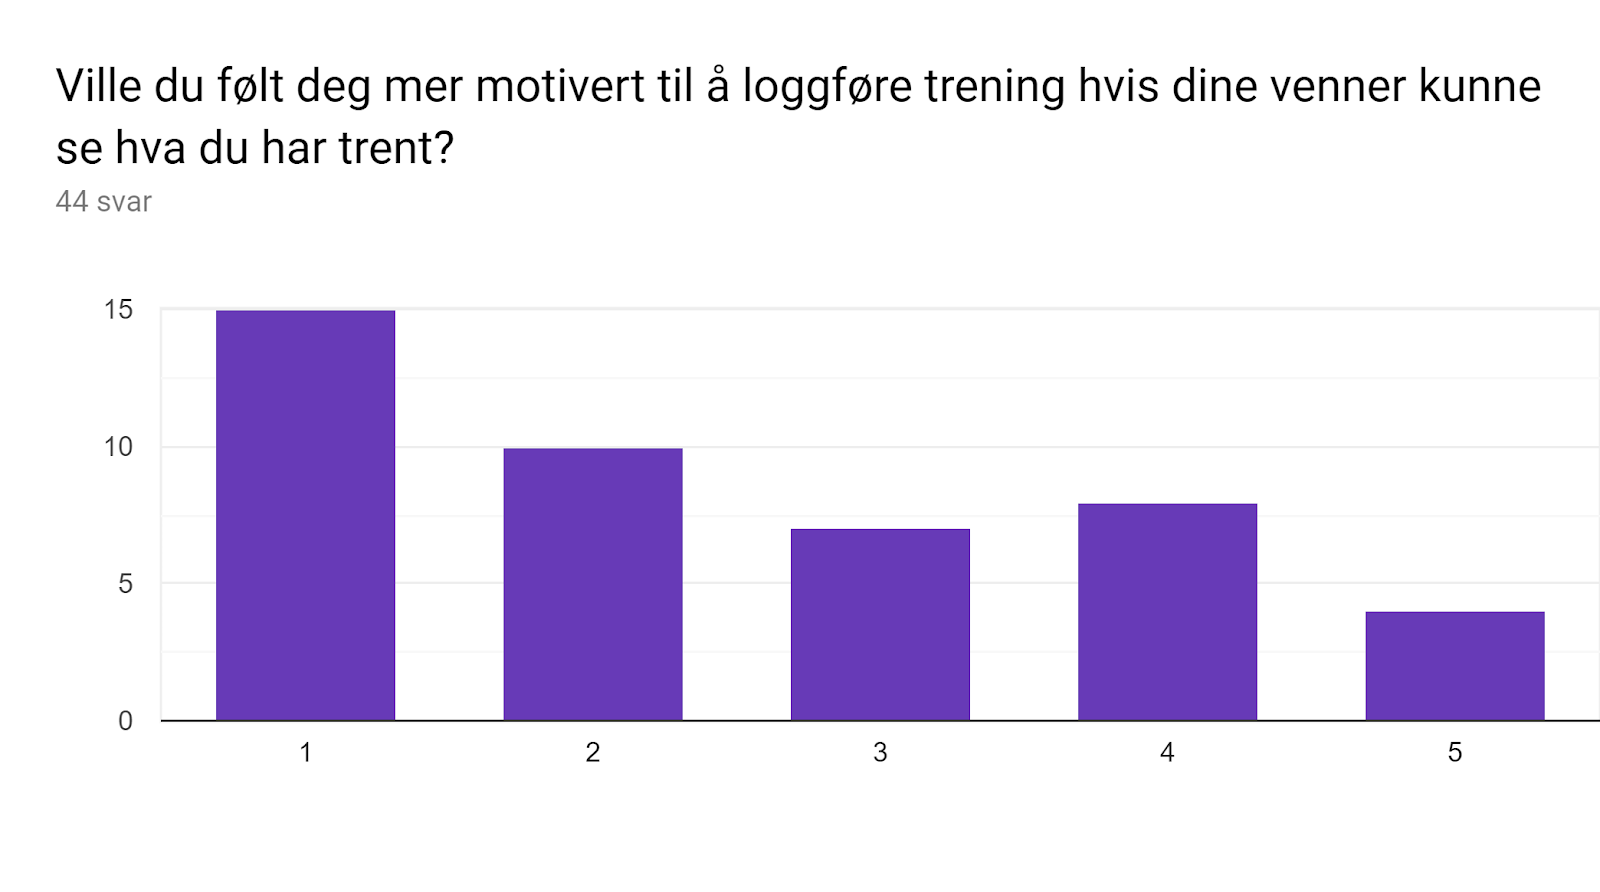
\includegraphics[width=120mm]{figures/MotivertTilLogging.png}
    \caption{Motivated to log workouts if friends could see the logs}
    \label{moti}
\end{figure}

The next question was about accountability and whether or not they would feel accountable to log their workouts if their friends could see them. The answers from figure \ref{acc} were almost identical to the motivation answers shown in figure \ref{moti} where the people mostly disagreed with the statement.

\begin{figure}[H]
    \centering
    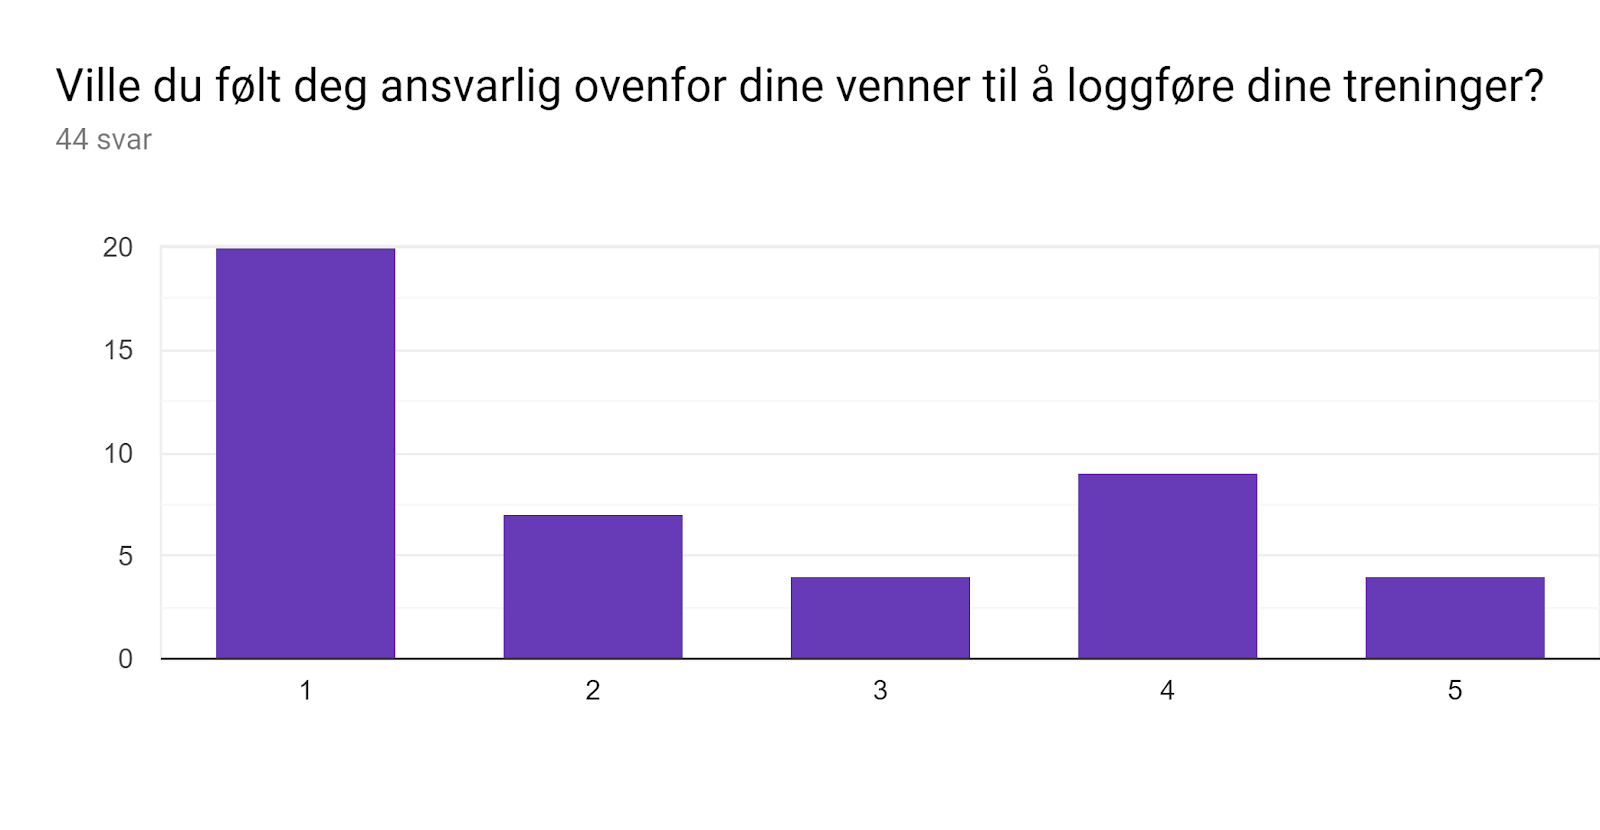
\includegraphics[width=120mm]{figures/AnsvarligLogging.png}
    \caption{Accountability from friends to log workouts}
    \label{acc}
\end{figure}
To find out if the surveyed people are interested in their friends workouts, they were asked if they were interested in friend`s progression in running, or if their friends gathered for a football game. The answers were quite mixed as shown in figure \ref{inti}, however the answers mostly disagreed with the statement. 
\begin{figure}[H]
    \centering
    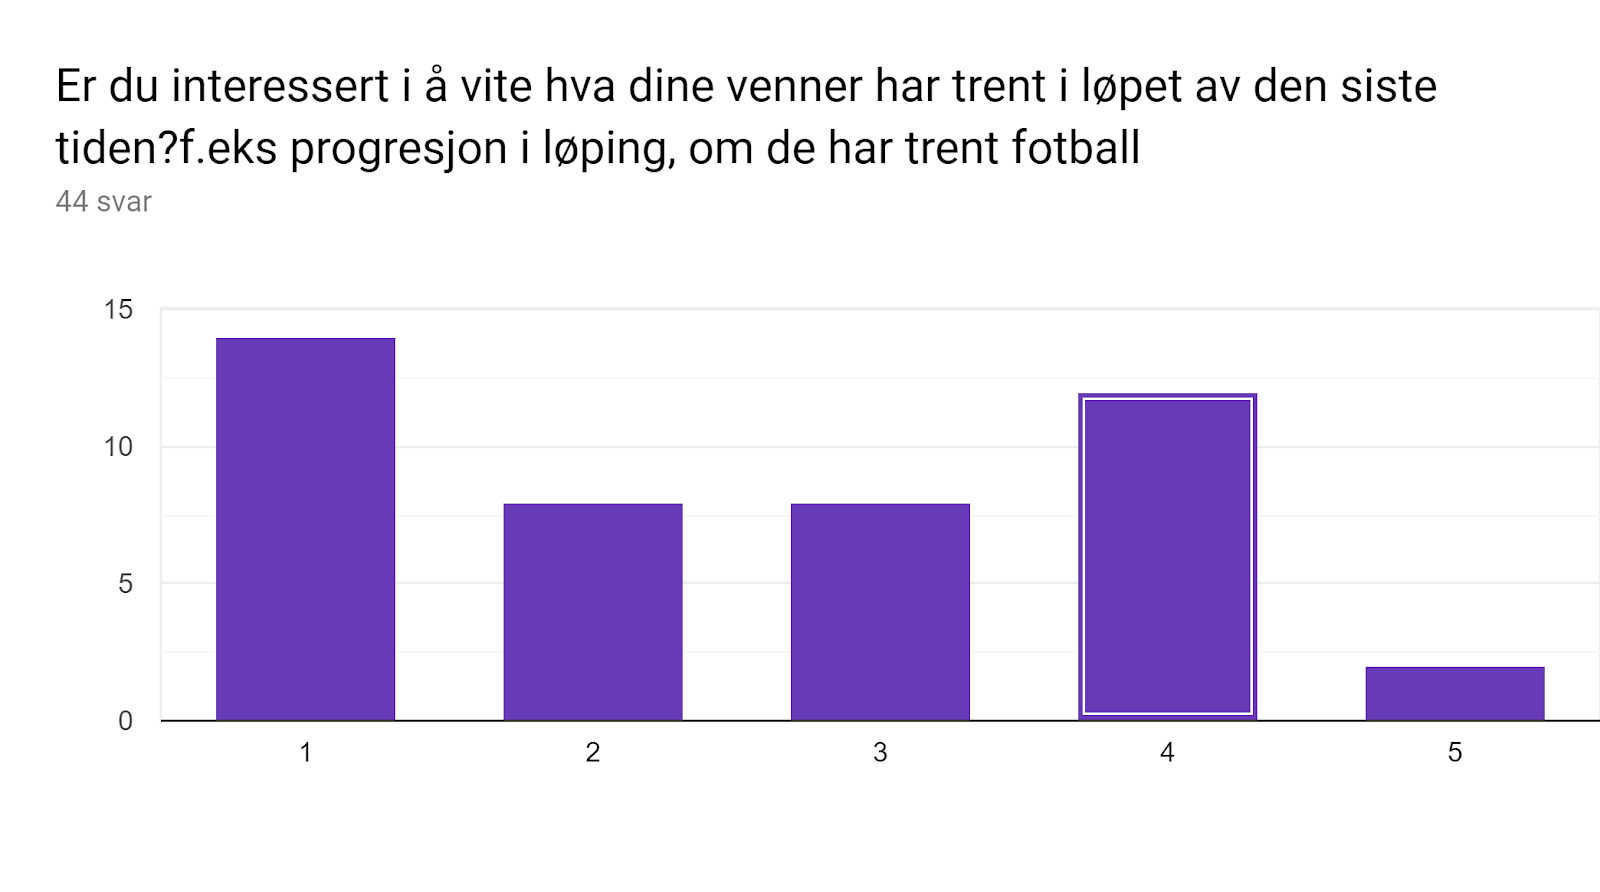
\includegraphics[width=120mm]{figures/AndresTrening.png}
    \caption{Interested in friends workouts and progress}
    \label{inti}
\end{figure}

As suggested in the literature review, having common goals is important to both stay motivated and accountable. The survey asked if it would be extra motivating to have a common workout goal that they co-operate with their friends. Examples would be running 5 kilometers together, lifting weights together or daily step challenges. The answers were mostly positive as seen in figure \ref{cgs}. Only 7 answers disagreed or strongly disagreed.
\begin{figure}[H]
    \centering
    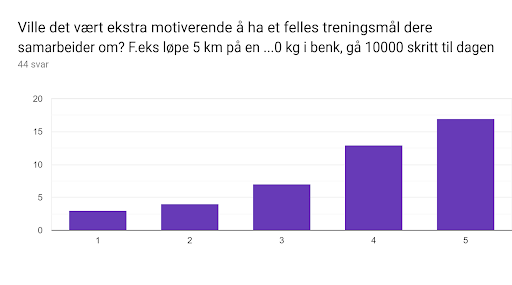
\includegraphics[width=120mm]{figures/FellesMaal.png}
    \caption{Motivation from common goals}
    \label{cgs}
\end{figure}
As a follow up to the last question, the surveyed people were asked if it is motivating to compete with friends towards a common goal. Again the answers were mostly positive to the suggestion as most people strongly agreed with the statement. 


\begin{figure}[H]
    \centering
    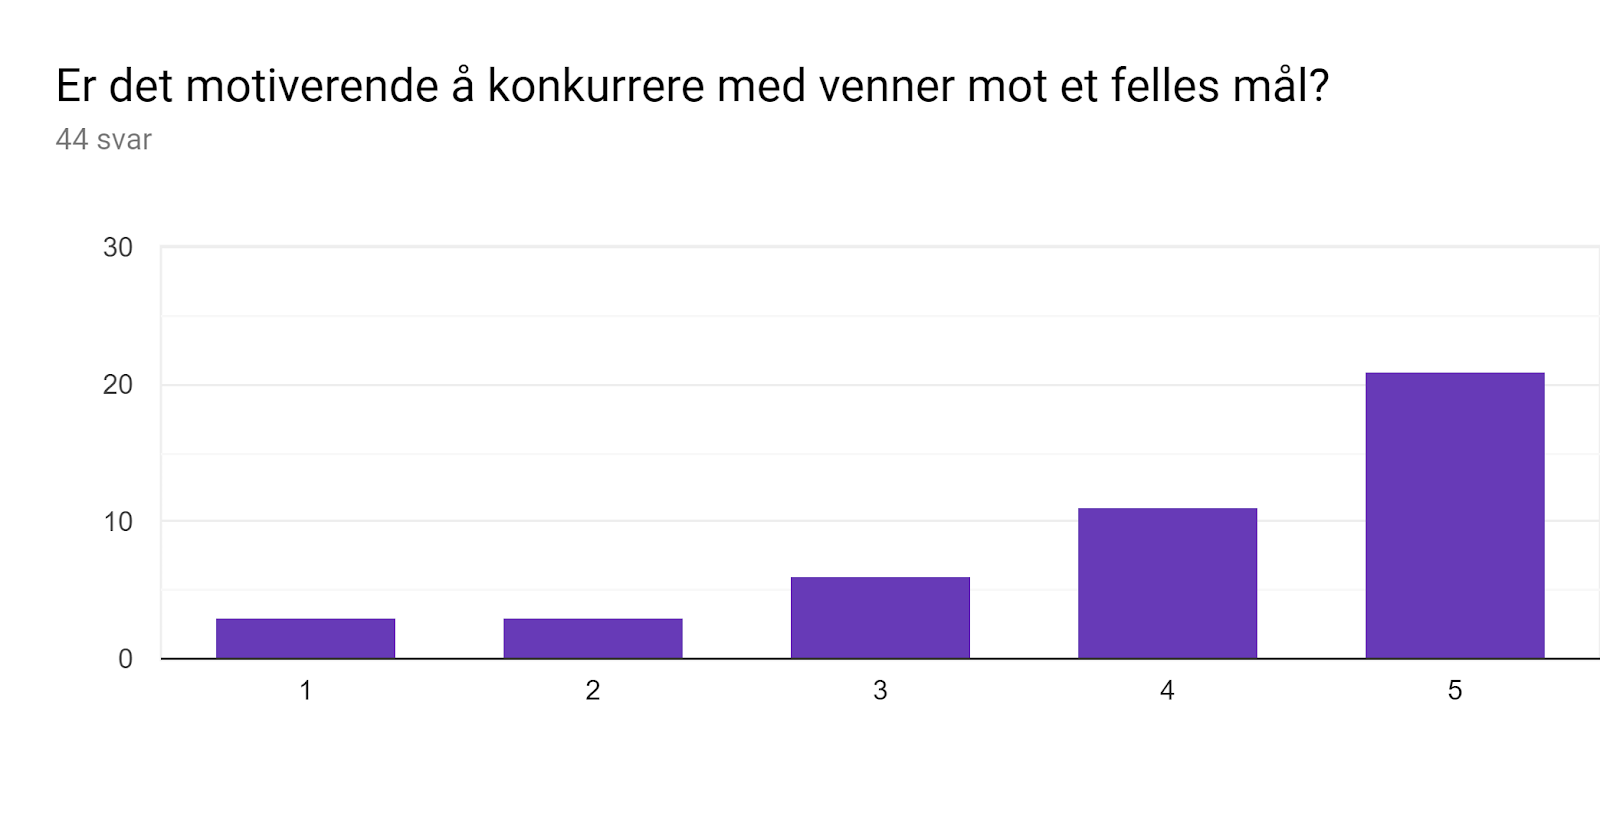
\includegraphics[width=120mm]{figures/KonkurereVenner.png}
    \caption{Competing with friends}
    \label{data}
\end{figure}
To get an idea of how members of a group would interact with each other, they were asked if they would like to get instant notifications if a member of their group was working out. The idea here is that if a member is working out at the moment, it would motivate the rest of the group to go out and do a workout.
As seen in figure \ref{instaN}, the answers are mostly strongly disagree or neutral. They prefer to have an asynchronous application instead of a synchronous application with push warnings or instant notifications.
\begin{figure}[H]
    \centering
    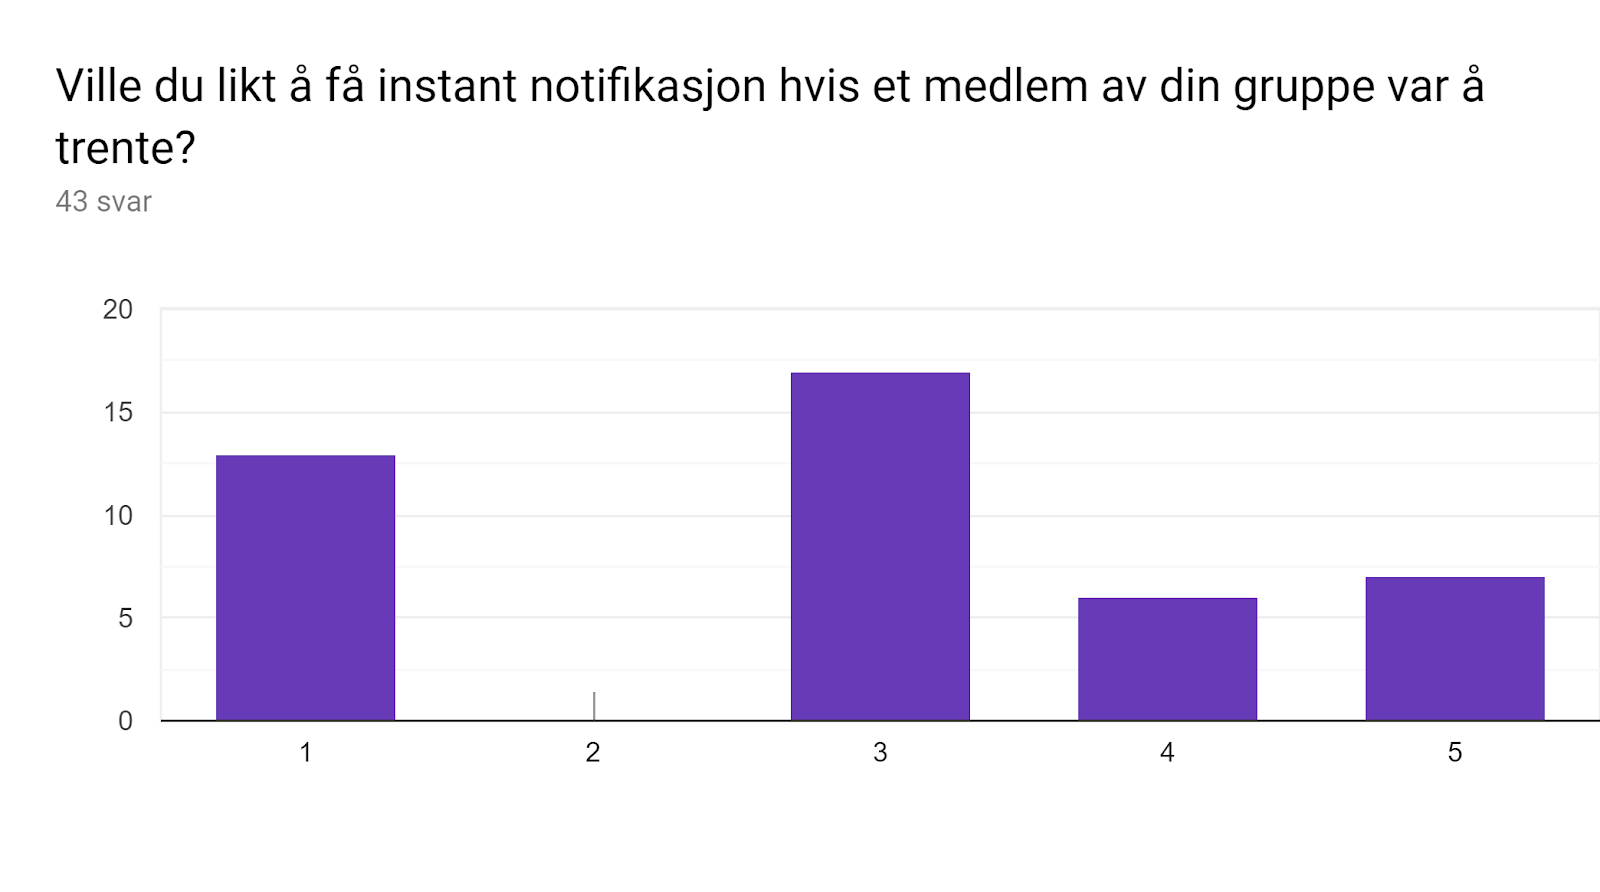
\includegraphics[width=120mm]{figures/InstantNotifikasjon.png}
    \caption{Instant notifications}
    \label{instaN}
\end{figure}

\begin{figure}[H]
    \centering
    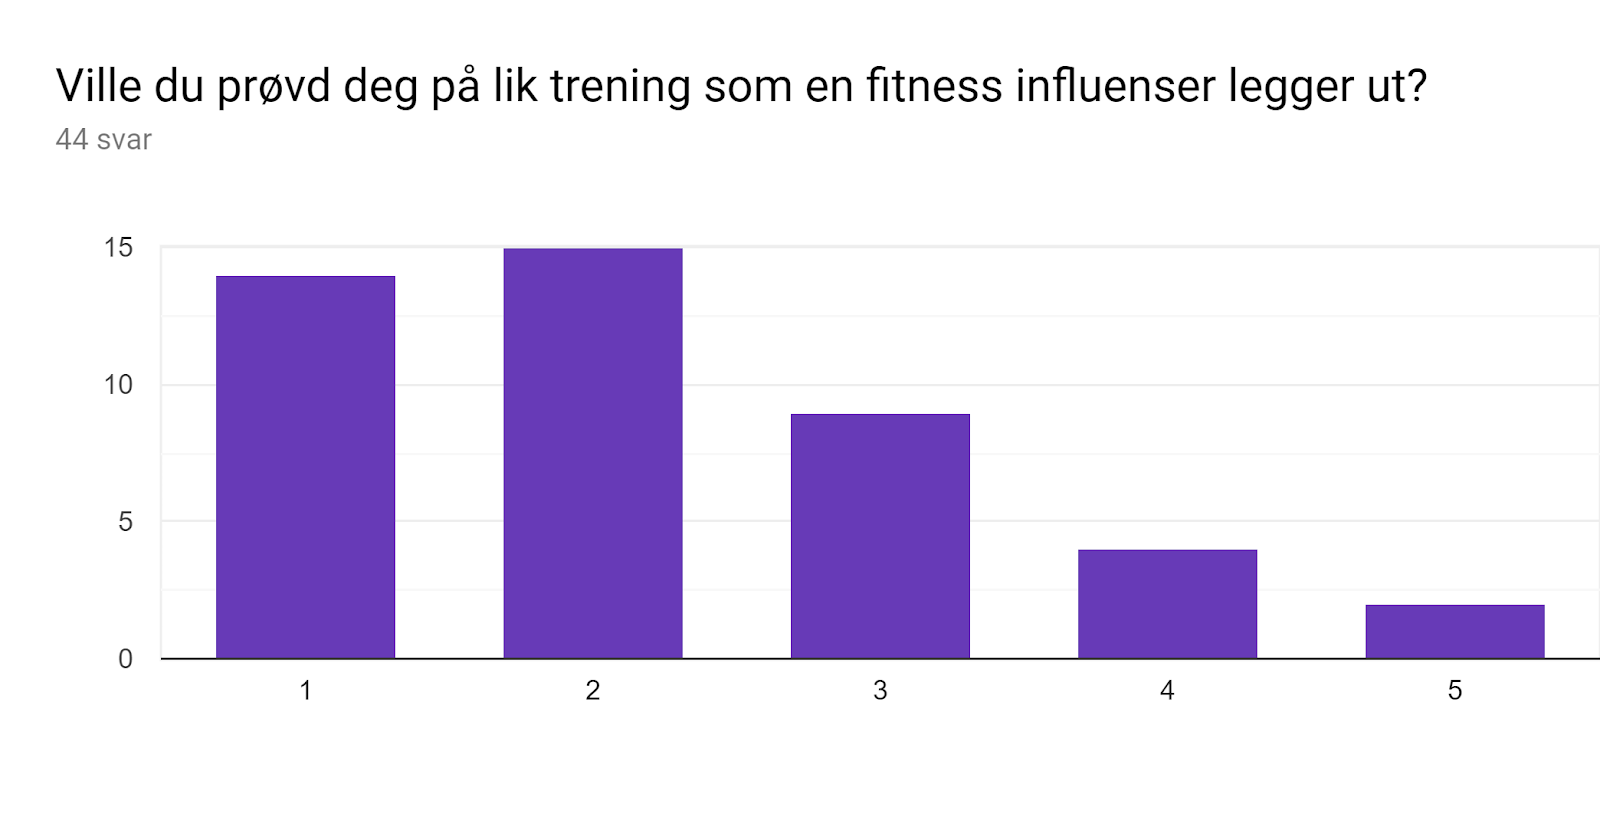
\includegraphics[width=120mm]{figures/FitnessInfluencer.png}
    \caption{Testing workouts from fitness influencers}
    \label{fitnitsinf}
\end{figure}
From the literature review it is suggested that some people take the role of a mentor and having mentors help people in the early stages by sharing information and knowledge. Fitness influencers are people that share exercises and workouts online on social media like Instagram and Snapchat. However the answers were negative and most people disagree that they would try the same workouts as fitness influencers share on social media. 
\begin{figure}[H]
    \centering
    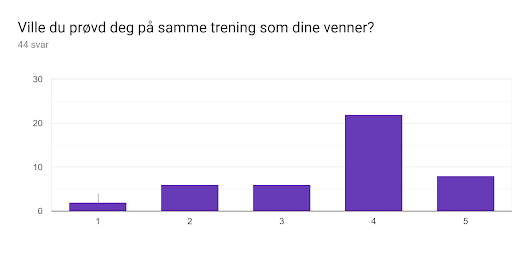
\includegraphics[width=120mm]{figures/VennerInfluencer.png}
    \caption{Testing workouts from friends}
    \label{fwork}
\end{figure}
As a follow up to figure \ref{fitnitsinf}, it is interesting to find that people much rather prefer to copy workouts from friends. Figure \ref{fwork} shows that people would like to try a workout written by a friend.
\subsection{Low-fidelity prototype}\label{lowfi}
The first version of the application was created as a sketch on paper. Several iterations were drawn on paper to test different layouts and features. The sketches were focused on the functionality of creating or joining groups and how to select and share goals. There is a workout logging feature that lets users log their own workouts and look at past workouts and a feature that lets the users look at the group members workout as well. The goals are selected by the group members and will be visible in the social group member part of the application. 
\begin{figure}[H]
    \centering
    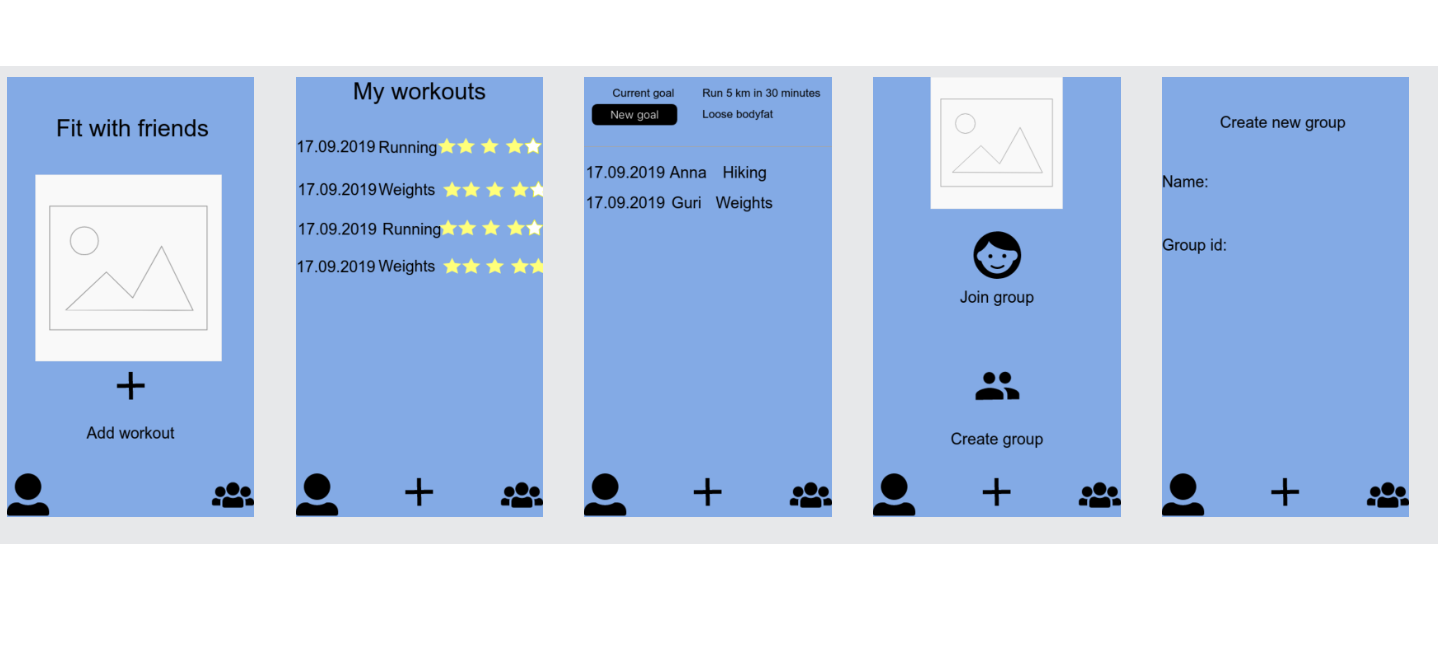
\includegraphics[width=120mm]{figures/testytestings.png}
    \caption{Wireframes for the application}
    \label{wireframe}
\end{figure}
Figure \ref{wireframe} shows some of the screens from the first wireframe that is created in the prototype program Proto.io. The bottom buttons on every screen are inspired from other social media applications. The user icon will go to your own workout log(the second screen) and the group of users will go to a group screen(the third screen) with the common goals and the other users workouts. The Add icon will be for adding workouts. The fourth and fifth screen shows the group screens, where the users will be able to join or create groups, select names for the group and then adding common goals for all their members.
\subsection{Interactive prototype}
With proto.io it is possible to add interactions and clickable buttons for the wireframes. This was used to create the first interactive low-fidelity prototype. The interactive prototype displayed the functions mentioned in section \ref{lowfi}. Instead of adding dropdown menus and clickable lists the features were presented with symbols and descriptive information to illustrate the different functions. Illustrative images were also added to improve the user experience of the low-fidelity prototype.
\begin{figure}[H]
    \centering
    
\includegraphics[scale=0.25]{figures/777.png}
    \caption{First interactive prototype with Proto.io}
    \label{intProt}
\end{figure}
\subsection{Expert interview} \label{expertinterview}
Two experts were interviewed at City Sammen, a physiotherapist and researcher and a developer, both work as personal trainers online and have worked with clients in person before. There was a brief introduction of the goals and ideas of the project, then the experts were introduced to the literature review and the answers from the survey. After a semi-structured interview was done with a set of pre-defined questions about how the personal trainers work, and the development and features of the application. 

The experts thought it was an interesting project and both agreed that setting personal goals and providing feedback and accountability is very important to keep improving the physical fitness of their clients. They also believed that having groups would increase the competition between the users and that it would keep the users accountable by "shaming" each other if they fell off.
One expert requested a way of visualising the progress towards a goal, with a progress bar or showing the progression percentage. Since it is important to show the progress that the users have made. Giving positive feedback like "great work", when a user logs their workout would be beneficial for accountability. At the end of the semi-structured interview there was a discussion between the experts about notifications. One of the experts recommended that having notifications with motivating quotes and telling the users that another user just worked out could help for the competition aspect, however the other expert agreed with the survey answers and thought that very few users would approve of this functionality. One of the experts also recommended creating the functionality in ReactJS.

\subsection{Proof of concept}
After conducting the literature review and the survey it was clear that there is a demand for group functionality for exercise applications and that it requires further research. The experts also liked the idea of an application with the proposed functionality for exercise accountability and exploring more design and technology solutions.

\section{Second Iteration of Research Project}
The second iteration consisted of changing the framework to ReactJS. This was done to test the functionality with a more realistic framework than a prototyping framework. Creating a new low-fidelity interactive prototype and implementing the current functionality there. The requirements were also redefined based on the feedback from the experts. Lastly a group of usability experts performed a SUS evaluation.
\subsection{Redefining after the expert feedback }
After the semi-structured interview with the experts some changes were made. The prototyping framework proto.io was switched with ReactJS, as an expert recommended it and it is one of the most popular frameworks for development.  The change required some learning time. 
The progress bar functionality for the group goals was also emphasized in this design iteration.

\subsection{Focus group} \label{focusgroup}
The focus group consisted three males(A,B,C) and one female(Z), who are all close friends. They were introduced to the research and were told about the ideas from the literature review. The goal of the focus group was to get the group to discuss what features and content they would like to see and most importantly stay accountable.
They were first asked if they use any fitness applications or if they have used any in the past. Two of them had used Fitbit and one had used Myfitnesspal. They had abandoned the applications because they were "boring", "not interesting" and the fun of the application quickly ended.

They were then asked if there are any features that would make them use a social fitness application.
\begin{itemize}
\item A: Having long-term goals with workout programs included, the ability to make bets with friends.
\item Z: Goals for workout frequency, general goals for working out a couple of times a week 
\item B: Competing with friends to win prizes, where the members put in money for weekly competitions. Competitions could be going to the gym the most times, working out the longest or doing the most total weight in a week. He mentioned that the application could have GPS locations for gyms, and that it should only be possible to log workouts from the gym. He also thought that having positive feedback when you log a workout is a nice touch, and the other group members should get a notification in the application when a member has logged a workout.
\item C Said that he exclusively works out alone and does not think that a social application would get him to log his workout or be interested in what his friends are doing.
\end{itemize}

The next part was dedicated to visualisation of the goals. They all agreed that the visualisation should be focused on the smaller goals, for instance having 10 workouts in total during a week for the group where every member has to contribute.  They mentioned that the bigger goals like working towards completing a marathon, or hitting a 100 kg bench press should be a personal goal and this could be visualised with a percentage bar. The intermediate objective goals could be visualised with check marks, using a green check mark for success and a orange check mark for in progress.

For the last part of the focus group the members were shown the current mid-fidelity prototype created in React. They did a walk through of the application where they could log a workout and go through the current components that had filler content.
\begin{figure}[H]
\flushright
    
\includegraphics[scale=0.6]{figures/appenSaaLangt2.png}
    \
    \caption{Prototype shown to the focus group}
    \label{ReactProt}
\end{figure}

They were then asked about design preferences, they all agreed that having intuitive user interface and to stay social was the most important part. They thought the buttons were intuitive enough so that they understood quickly what would happen.
For the color preferences they agreed that light colors with dark text is the best option, and that it looked more professional without "aggressive screaming colors".
\subsection{Design principles}
In order to improve the prototype for testing, the five design principles were reviewed and integrated to the prototype design. For the visibility principle, text was added and replaced some of the content filler that was in "your workouts" and "your friends workouts", this added to the constraint and feedback principles as well as now it is easier to understand where in the application a user is and makes it harder to do mistakes.

For the feedback principle the navigation buttons now show a transition to the button that was pressed and the button changes colour to blue and is slightly bigger than the other two as shown in figure \ref{GruppeAss1}. The design is also consistent over every screen of the application with the same background colours, images, navigation and font. The same goes for the affordance principle as there are common icons and the layout which is inspired from social media platforms which matches the industry


\section{Third Iteration of Research Project}
For the third iteration, the feedback from the focus group was implemented to the prototype. A visualisation bar was added to the group workout to represent the personal goal of the user, and both the personal and group goals are shown as well. 
The prototype was evaluated by usability experts with SUS and a group survey.

\subsection{SUS and survey with Usability Experts}
The evaluation of the third design iteration was conducted by six people. The usability experts were divided in to groups of three to get a feeling of the social aspect of the prototype. They were told about the previous iterations of the research project and answered a survey after doing the SUS analysis.
\begin{figure}[H]
    \flushright
    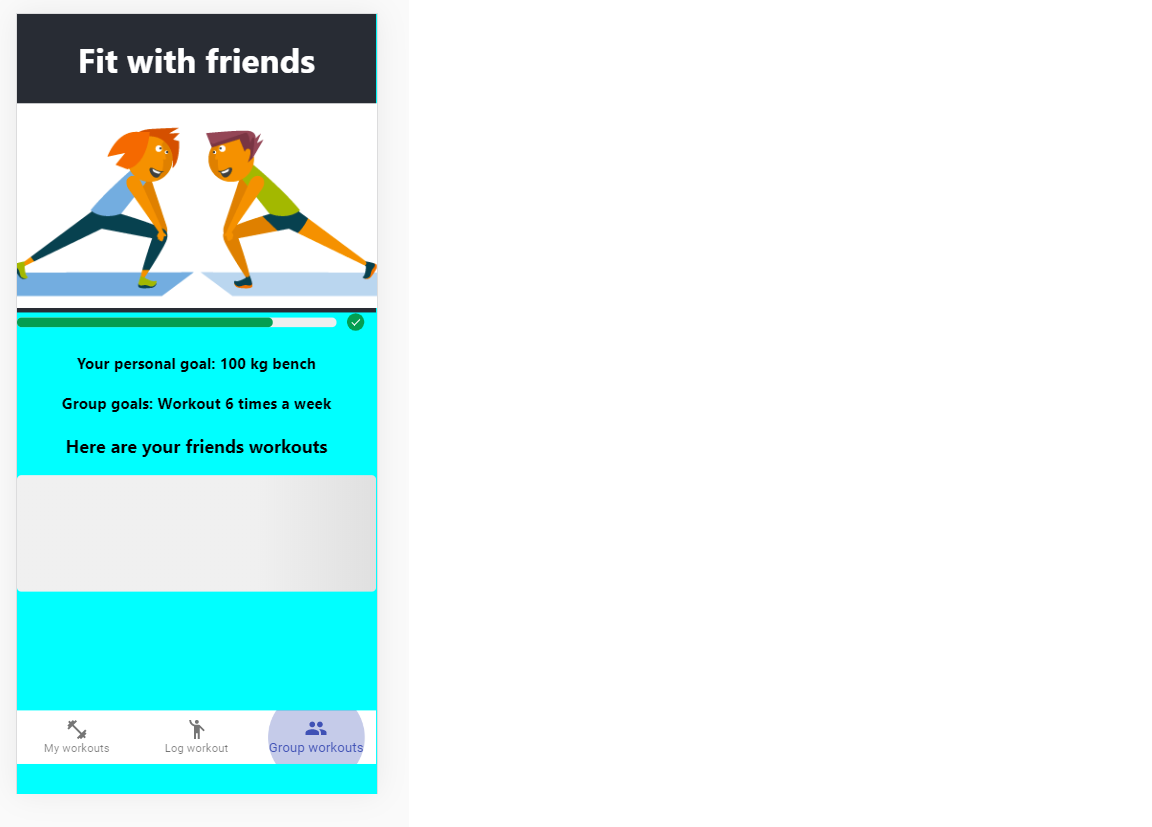
\includegraphics[scale=0.6]{figures/GruppeAspekt1.png}
    \caption{Prototype with progress bar, goals and content}
    \label{GruppeAss1}
\end{figure}

The prototype \ref{GruppeAss1} was shown to the usability experts on a laptop screen with a responsive layout window of an iPhone X. The evaluating experts consisted of six information science master students. They were guided through the prototype and explained the basic functionality of the application and how the social features would work. The experts had then a couple of minutes to click through the prototype and after they evaluated the prototype with SUS and a quick group survey.
The first group gave an average score of 90,8 and the second group gave an average score of 93,3, which is considered as best imaginable. The score might be inflated as the evaluating experts know about the SUS from beforehand and wanted to be nice.

\subsection{Group survey}
Each group conducted a group survey about the functionality after completing the SUS. They were asked three questions that prompted a discussion. 
Question 1: Is there any functionality that you and your group thinks is missing?
\begin{itemize}
    \item Group 1: Would love to have a graph showing the progression towards the personal goals.
    Likes when the data is visualised, how much weight has been lifted in a gym session, how far you have run each workout and if there is progress.
    \item Group 2: Being able to log diet and share what you have eaten today, having a caloric calculator and show how many calories you have approximately used per day. One of the members pointed out that the progress bar should be below the personal goal, and the green checkmark should be changed since it looked like the goal was completed.
\end{itemize}

Question 2: Would your group be interested in having a leaderboard in the group section that would show which member is working out the most each week or month?
\begin{itemize}
    \item Group 1: Yes to both, really think both would help motivate the group members and all of them thought that it would help them to stay more active.
    \item Group 2: Yes, very motivating and would love to have a weekly rapport showing who is on top and what the members have done.
\end{itemize}

Question 3: Would you use a fitness application with the social functionality? ( Assuming your group of friends would too)
\begin{itemize}
    \item Group 1: Yes and "yes if I actually worked out or my friends guilted me into doing it"
    \item Group 2: Yes absolutely, especially if our friends joined.
\end{itemize}


\subsection{Redefining after feedback from usability experts}
After the feedback from the usability experts, a leaderboard was implemented to the prototype as well as a few design changes in the group section, the goal was moved above the progress bar, and the progress bar visualisation was changed so that the green checkmark only shows if the progress is complete, and the bar now is blue and shows that the goal is active.

\section{Fourth Iteration of Research Project}
The fourth iteration of the prototype consisted of testing the prototype with two users. The users evaluated the prototype with SUS and a usability test. The prototype was evaluated by experts with Nielsen`s heuristics as well.

\subsection{SUS with users}
A SUS evaluation was conducted by two users that contributed to the survey and the usability testing after. The users are economy students and are regular users of fitness applications.
They were shown the prototype on a laptop with iPhone X viewport and were allowed to click around to test the functionality and did three usability tasks before evaluating with SUS. Both users gave a SUS score above 90 which is seen as best imaginable and shows that the design of the prototype is intuitive and easy to use.

Additional feedback from the test users suggested adding search functionality for exercises and a calendar to easier portray the days you worked out and what you did for your workout. The results of the SUS can be seen in section \ref{susu}.

\subsection{Usability testing with users}
The participants of the usability test performed three different tasks. The tasks were performed on a laptop with iPhone X layout and were timed on every task they were given. The participants were quickly introduced to the functionality of the prototype and the research before the task, and then had some time to navigate around. The participants were presented with four different tasks that would be timed.
The users did not make any mistakes and the user interface and design seemed intuitive and easy to use. The results are shown in section \ref{usat}.

\subsection{Heuristics with experts}
Three usability experts were contacted to evaluate the prototype with Nielsen`s heuristics. The users were shown the high-fidelity prototype on a laptop with an iPhone X layout. The results are shown in section \ref{heur} .


\section{Future iterations}
After conducting the user and expert testing there were suggestions for new functionality that could be implemented in a future iteration. One suggestion was to add comments on your own workout and friends workouts to add to the social features and make it more of a social network feeling. Another suggestion which would be hard to implement was to add the data from fitness trackers to the applications or get the daily steps counter from the mobile phones of the users.  From the heuristic evaluation there are a few major usability problems that should be prioritised as well. Letting the users change their goals and adding more than one goal and adding more error prevention and easy to understand messages if an error occurs. 





\chapter{Features of Fit with friends}
This is the overview of the functionalities from the high-fidelity prototype. This is the final product from this research project and the application consists of three different sections.

\section{Logging workouts}
The logging workout section is the front page of the application. The bottom navigation includes "My workouts" , "log workout" and "Group workouts". Log workout leads to a user form that consists of three steps. In the first step of the form, it asks the user what kind of workout is being logged (gym, running, swimming or other) and the details of the workout. The next step asks the user to confirm the details and it is possible to go back to make changes.
\begin{figure}[H]
  \centering
  \begin{minipage}[b]{0.4\textwidth}
    
\includegraphics[width=\textwidth]{figures/loggingworkouts.png}
    \caption{Logging workouts}
  \end{minipage}
  \hfill
  \begin{minipage}[b]{0.4\textwidth}
    
\includegraphics[width=\textwidth]{figures/confirmworkouts.png}
    \caption{Confirming input}
  \end{minipage}
\end{figure}
The last step is the success form, the user gets a positive message "Great work" and "Your workout will be added to your log".
\begin{figure}[H]
    \centering
    
\includegraphics[scale=0.6]{figures/feedbackworkouts.png}
    \caption{Positive feedback}
\end{figure}

\section{My workouts}
My workouts is the personal log of the user. This section consists of all the personal data and information the user has logged in the application. The workout data is presented in tables with the format of exercise, weight, rep scheme. The logged data would show up for the users friends in their social section.
\begin{figure}[H]
    \centering
    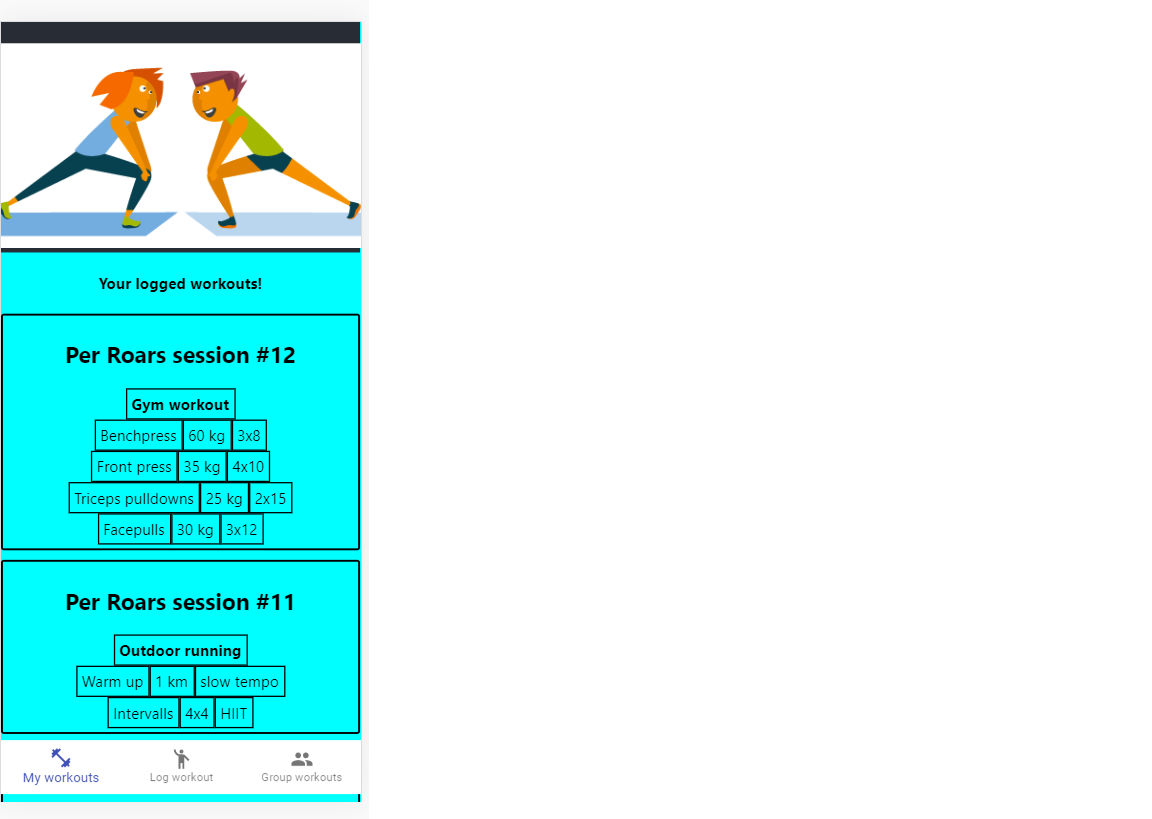
\includegraphics[scale=0.6]{figures/yourloggedworkouts.png}
    \caption{My logged workouts}
    \label{MYLog}
\end{figure}

\section{Social section}
Group workouts is the social section of the application. It includes a personal goal which is supposed to be a long term goal and displays the group goals which are short term goals for the group like going go the gym a total of 10 times a week.
The workout logs of every group member is shown in the social section, this functionality is hidden and if clicked returns a list consisting of all the recent workouts.
\begin{figure}[H]
    \centering
    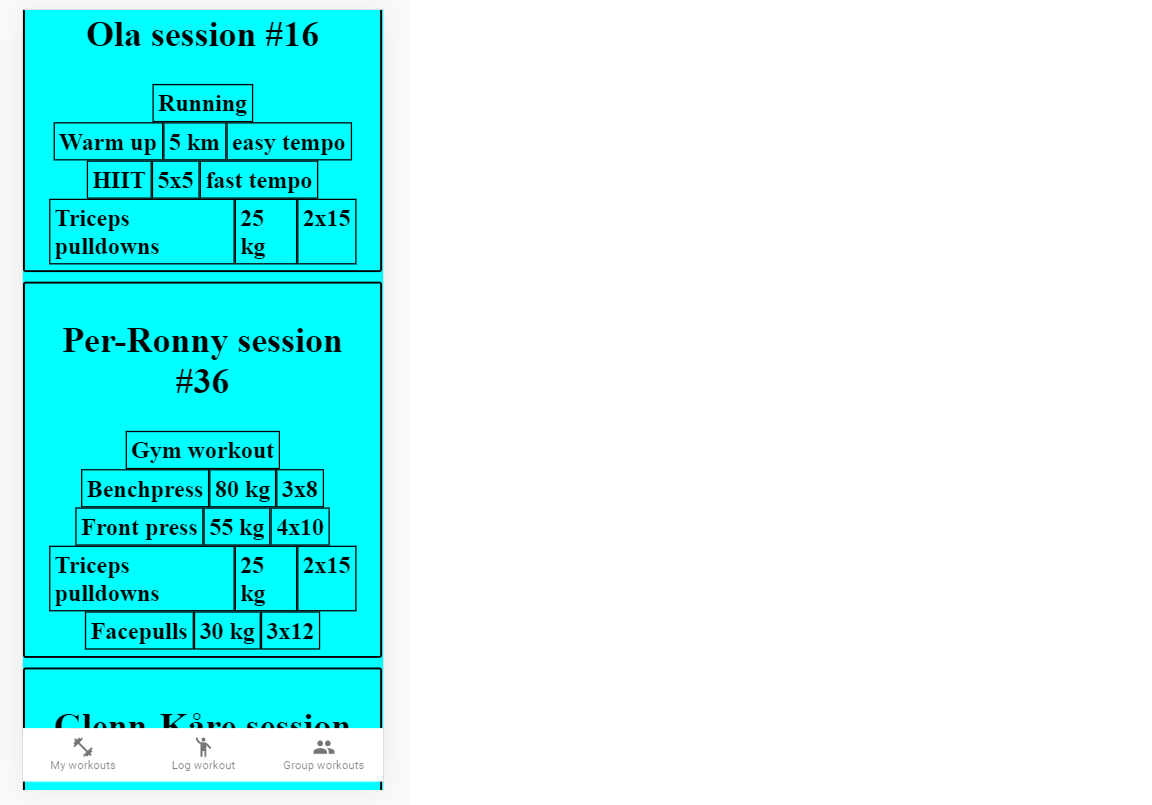
\includegraphics[scale=0.6]{figures/friendsworkoutlogs.png}
    \caption{My friends logged workouts}
    \label{FriendLog}
\end{figure}
This lets the users share information and knowledge about workouts which the users can copy or get inspired and motivated by.
\begin{figure}[H]
    \centering
    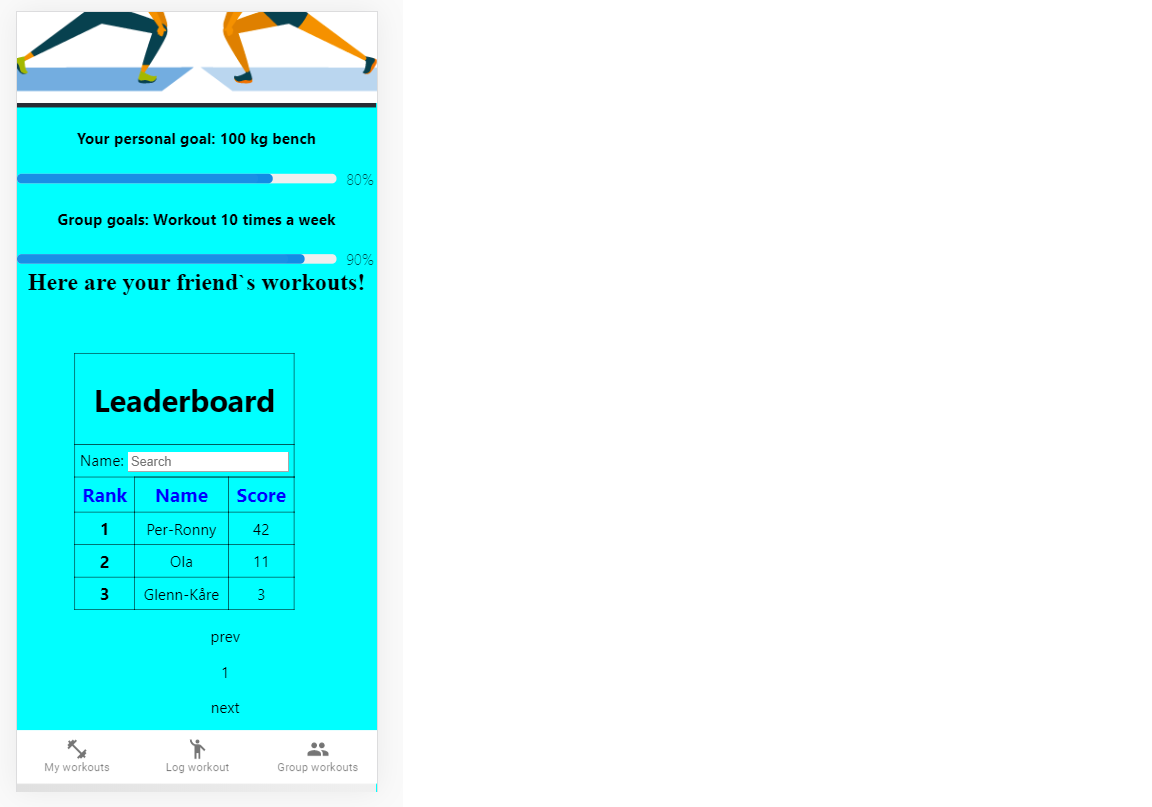
\includegraphics[scale=0.6]{figures/leaderboardandgoals.png}
    \caption{Leaderboard, goals and toggleable friend workouts}
    \label{LeaderB}
\end{figure}
The leaderboard is a gamification design to encourage the group members to compete with each other, a user would get a point if they log a workout and the points form a rank to see who has the most points. The weekly leader would get a notification stating that they have won and then the leaderboard would reset so the users are competing on fair terms every week for their goal.




\chapter{Evaluation}
This chapter presents the evaluation results of the different design iterations from the SUS, usability testing and Nielsen`s heuristics.

\section{Participants}
Different groups evaluated each design iteration and the project switched between usability experts and intended users. The first group that participated in a focus group consisted of intended users who were a group of friends with a similar fitness level and were all motivated to improving their fitness levels. The other groups were usability experts who have all gotten a IT related degree and have participated in courses with interaction design and human-computer interaction.

Fyr opp noen tabeller med litt snitt ting på test?

\section{System Usability Scale}
The usability experts evaluated the application first with a system usability scale (SUS) method. The experts evaluated the prototype on a laptop screen with an iPhone X layout. The intented users evaluated the prototype on a ..

\section{SUS with Experts}
The usability experts did the SUS evaluation during the third design iteration with a mid-fidelity prototype with some functionality implemented. The usability experts returned an average score of 92. The experts answered the survey individually and were in the same room.
\section{SUS with Users}\label{susu}

\section{Usability Testing}\label{usat}
Two users were prestented with three different tasks and were timed to find out how effective and efficiently they could use the prototype. The users were not given any instructions on how to solve a task, however they had prior knowledge about the prototype as they evaluated it with SUS. 
Noticeable differences in users?

U1

u2

Task 1 was to find a prior workout??

Task 2, change goals??

Task 3, find friends workout??

\section{Heuristics with experts}\label{heur}
Nielsen`s heuristics was used as the last step of the fourth design iteration. Two/Three information science masters students evaluated and tested the high-fidelity prototype. The evaluators were prestend the prototype on a laptop with iPhone X layout and evaluated the prototype seperately. Below is the condensed feedback for all of the ten heuristics.

\textbf{1. Visibility of System Status:}

\textbf{2. Match between the System and the Real World}

\textbf{3. User control and Freedom}

\textbf{4. Consistency and Standard}

\textbf{5. Error provention}

\textbf{6. Recognition rather than Recall}

\textbf{7. Flexibility and Efficiency of Use}

\textbf{8. Aesthetics and Minimalistic Design}

\textbf{9. Help Users Recognise, Diagnose, and Recover from Errors}

\textbf{10. Help and Documentation}



\chapter{Discussion}
\section{Methodologies}
\subsection{Design Science Research}
\subsection{Design Principles}
\subsection{Data Gathering}
\subsection{Evaluation of Prototypes}
\section{Prototype Development}
\section{Limitations}
\section{Research Questions}

\chapter{Conclusion and Future Work}
\section{Conclusion}
\section{Future Work}
\subsection{Maintaining fit with friends}
Maintaining an application is important for the application to survive and stay relevant. As more technological devices are created for the fitness industry to gather data and information it is important to find a valuable way to represent the data. The functionality from fit with friends could be incorporated with  popular fitness application to make them social which would let the users interact more with each other. This would be the best case to let developers implement the features and use their own design. The application should be available in Google play store or iTunes to make the functionality visible to potential users. 

\subsection{New features}

groups,
chat, 
diet,
caloric estimates,
cookie cutter programs



% Include more chapters as required.
%%=========================================
\renewcommand{\glossarypreamble}{\footnotesize}
\printglossary[style=super, type=\glsdefaulttype] \let\cleardoublepage\clearpage
\printglossary[style=super, type=\acronymtype]
% Include more appendices as required.
%%=========================================
\clearpage
\DeclareRobustCommand{\VAN}[3]{#3}
\addcontentsline{toc}{chapter}{Bibliography}
\bibliographystyle{generators/myplainnat}
\bibliography{generators/refs}
\appendix
\titleformat{\chapter}[display]
  {\normalfont\large\bfseries}% <- font for label "Appendix A", default \huge
  {\chaptertitlename\ \thechapter}
  {20pt}
  {\large}% <- font for title, default \Huge

\section{Appendix A}

\section{A 1 -Approval from NSD}

\includepdf[pages=-]{pdfAppendix/NSD.pdf}


\section{Appendix B}
\section{B 1 - Informed consent form}

\includepdf[pages=-]{pdfAppendix/InformasjonsSkriv.pdf}

\section{B 2 - Interview guide for experts}

\includepdf[pages=-]{pdfAppendix/expertGuide.pdf}

\section{B 3 - Interview guide for users}

\includepdf[pages=-]{pdfAppendix/groupGuide.pdf}
\section{B 4 - System usability scale form}
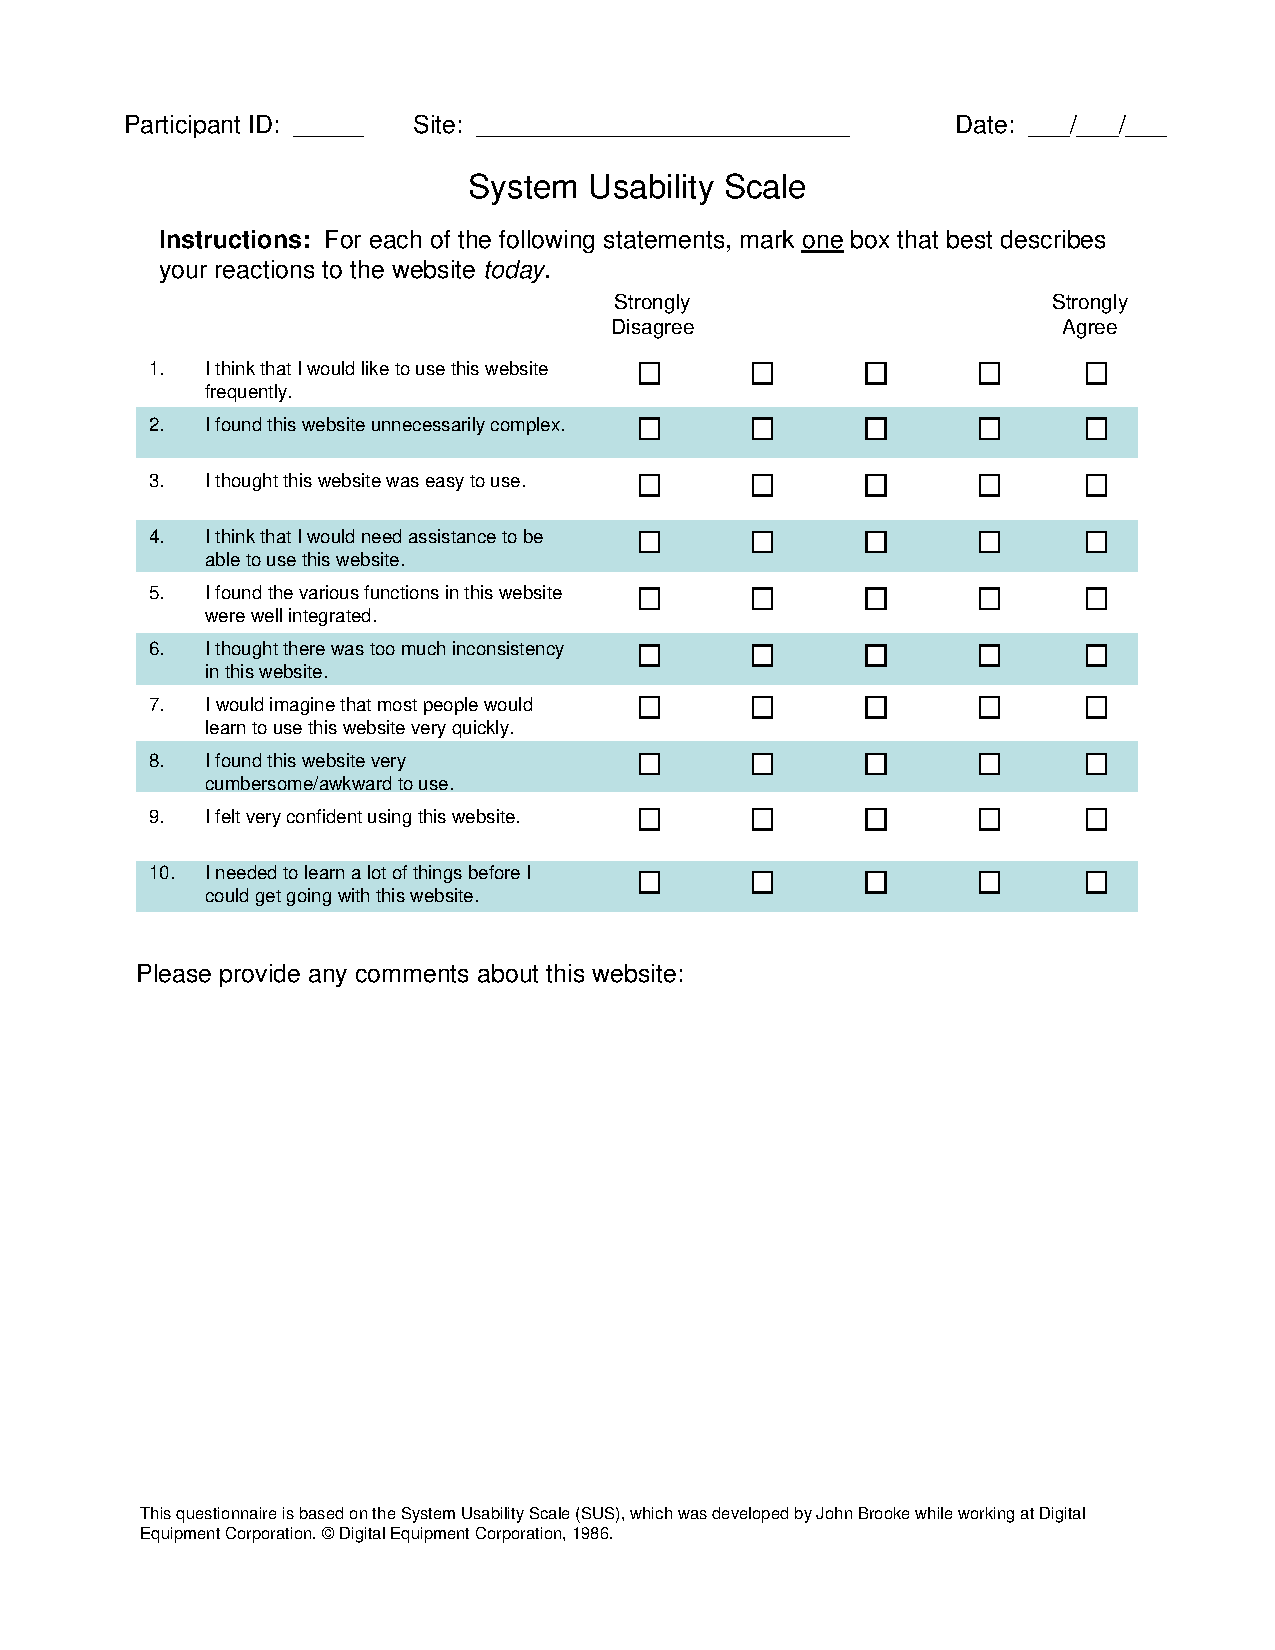
\includepdf[pages=-]{pdfAppendix/SUS.pdf}

\section{Development tools}
\subsection{Proto.io}
Proto.io is an application prototyping platform \cite{proto} that can can simulate everything an app can do. That includes interactive touch gestures, screen transitions and animations. It allows users to create realistic, shareable prototypes that work as a real app should and experience their prototype on the actual device.
\subsection{ReactJS}
ReactJS is a javascript library for building user interfaces \cite{react}. It is a flexible and efficient front end javascript library for building user interfaces\cite{react2}. ReactJS is developed by Facebook and is used by a variety of websites and applications. 

\subsection{Google forms}
Google Forms is a tool that allows collecting information from users via a personalized survey or quiz. The information is then collected and automatically connected to a spreadsheet\cite{forms}. Google forms was used to create a survey that was shared on social media, which helped gather valuable information.
\subsection{Atom}
Atom is the text-editor that was used to code in for this project. With atom it is possible to import packages, have multiple panes, manage packages and helps you write code faster with a smart and flexible autocomplete \cite{atom}.   
\subsection{Github}
Github provides software development version control using git. It provides access control and several collaboration features such as bug tracking, feature requests, task management, and wikis for every project \cite{github} . 
\end{document}